% =============================================================================
% Presentación del proyecto final de Computer Vision (grupo 3): TurtleBot 4, Tareas A y B.
% Plantilla y estilo: presentacion_referencia/ (portada slate-blocks + tema minimalista en estilo/).
%
%   (distrobox) python presentacion/scripts/carrera_con_ruta.py --mundo tubo:3 --turbo --video v.mp4 -> figuras/datos/
%   (distrobox) python presentacion/scripts/figuras.py v.mp4                               -> figuras/gen/ (y fotos del informe)
%   cd presentacion && latexmk -pdf presentacion.tex   (dos pasadas: la portada usa remember picture)
%
% 10 diapositivas para 10 minutos (pedido: máximo 10 y solo lo esencial): una figura central por
% diapositiva y 2-3 datos clave. Cubre lo que pide el enunciado: arquitectura, sensores, reconocimiento
% facial, gestos (Tarea B), navegación autónoma (Tarea A), decisiones, resultados y lecciones.
% Todos los números salen de los README del repositorio, de docs/pruebas_simulacro.md (robot real,
% 19/11), de scripts/figuras.py (simulador, reconocimiento sobre la cámara real del robot) o de las corridas
% del 22/11 con el código de la meta con bandera (banco_pruebas.py tubo:1..32 --turbo: 32/32; --duro: 13/16;
% reconocimiento.evaluar con y sin espejo, 1320 cuadros por tamaño).
% La competencia es el mismo día de la presentación: no hay resultados de la competencia en las diapositivas.
% =============================================================================
\documentclass[aspectratio=1610, 11pt]{beamer}
% =============================================================================
% tema.tex — aspecto de todas las diapositivas salvo la portada.
%
% Mismo estilo que presentacion_referencia/estilo/tema.tex (plantilla PPGE-UCB adaptada): fondo blanco,
% título arriba a la izquierda sin barra, sin cabecera, pie con una franja gruesa (morado) y otra fina
% (celeste), navegación por secciones con un punto por diapositiva y número de diapositiva a la derecha.
% Estilo minimalista: texto en gris oscuro (cInk) y gris (cSrc), un solo acento (cAcc) para títulos y
% cifras clave; los colores de los datos solo en las figuras.
%
% Cambios respecto a la referencia: colores de los estados de la carrera (IDA, FILA, QR, VUELTA), estilos
% TikZ de las figuras del robot, pgfplots para los gráficos, y el dibujo del cierre es el circuito
% (cajas, una señal, fotos con QR y el robot) en lugar de las edificaciones.
% =============================================================================
\usepackage[T1]{fontenc}
\usepackage[utf8]{inputenc}
\usepackage[sfdefault,lining]{FiraSans}
\usepackage[spanish,es-nodecimaldot,es-noshorthands]{babel}
\usepackage{graphicx}
\usepackage{amsmath}
\usepackage{booktabs}
\usepackage{array}
\usepackage{fontawesome5}
\usepackage{tikz}
\usepackage{pgfplots}
\pgfplotsset{compat=1.18}
\usetikzlibrary{positioning,arrows.meta,calc,fit,backgrounds,shapes.misc,shapes.geometric,babel}

% ---- paleta (la de la referencia) -------------------------------------------------
\definecolor{cPub}{HTML}{8A97EE}     % morado
\definecolor{cAcc}{HTML}{4F5FC8}     % morado oscuro (titulos, acentos)
\definecolor{cLight}{HTML}{00BFFF}   % celeste
\definecolor{cCelD}{HTML}{0090C8}    % celeste oscuro (texto sobre blanco)
\definecolor{cEncBg}{HTML}{DEE2FB}   % morado claro
\definecolor{cDecBg}{HTML}{D9F4FF}   % celeste claro
\definecolor{cInk}{HTML}{2E3140}
\definecolor{cOurs}{HTML}{D92626}
\definecolor{cOursD}{HTML}{9E1B1B}
\definecolor{cUni}{HTML}{E08A2E}
\definecolor{cUniD}{HTML}{A85E14}
\definecolor{cSrc}{HTML}{5A5D6E}
\definecolor{cMuted}{HTML}{8A8A96}
\definecolor{cRule}{HTML}{E2E3EA}
\definecolor{cPaper}{HTML}{F5F6FA}
\definecolor{cOk}{HTML}{3C9A5F}
% estados de la carrera (Tarea A), iguales en el circuito, la línea de tiempo y la máquina de estados
% solo dos colores en los diagramas (morado y celeste, con sus tonos claros); los demas son grises
\colorlet{cIda}{cAcc}
\colorlet{cFila}{cCelD}
\colorlet{cQr}{cLight}
\colorlet{cVuelta}{cPub}

% ---- estructura de la plantilla -------------------------------------------------
\useoutertheme[subsection=false]{miniframes}
\useinnertheme{rectangles}
\setbeamertemplate{navigation symbols}{}
\setbeamersize{text margin left=10mm, text margin right=10mm}

\setbeamercolor{normal text}{fg=cInk, bg=white}
\setbeamercolor{background canvas}{bg=white}
\setbeamercolor{structure}{fg=cAcc}
\setbeamercolor{alerted text}{fg=cOurs}
\setbeamercolor{frametitle}{fg=cAcc, bg=white}
\setbeamercolor{footline1}{bg=cPub}
\setbeamercolor{footline2}{bg=cLight}
\setbeamercolor{section in head/foot}{fg=cAcc, bg=white}
\setbeamercolor{mini frame}{fg=cAcc}
\setbeamerfont{frametitle}{size=\Large, series=\mdseries}
\setbeamerfont{section in head/foot}{size=\fontsize{6.5}{7.5}\selectfont}
\setbeamertemplate{itemize item}{\color{cAcc}\raisebox{0.2ex}{\tiny$\blacksquare$}}
\setbeamertemplate{itemize subitem}{\color{cMuted}\raisebox{0.2ex}{\tiny$\blacktriangleright$}}
\setlength{\leftmargini}{1.1em}

\setbeamertemplate{headline}{}

\setbeamertemplate{frametitle}{%
  \vskip 4mm
  {\usebeamerfont{frametitle}\usebeamercolor[fg]{frametitle}\insertframetitle\par}%
  \vskip 0.8mm
}

\makeatletter
\setbeamertemplate{footline}{%
  \begin{beamercolorbox}[wd=\paperwidth, ht=2.2mm, dp=0pt]{footline1}\end{beamercolorbox}%
  \begin{beamercolorbox}[wd=\paperwidth, ht=0.6mm, dp=0pt]{footline2}\end{beamercolorbox}%
  \begin{beamercolorbox}[wd=\paperwidth]{section in head/foot}%
    \vskip 2pt
    \hbox to \paperwidth{\insertnavigation{\dimexpr\paperwidth-14mm\relax}\hfill
      \raisebox{0.4mm}{\fontsize{6}{7}\selectfont\color{cSrc}\insertframenumber\,/\,\inserttotalframenumber}\hskip 5mm}%
    \vskip 3pt
  \end{beamercolorbox}}
\makeatother

% ---- piezas reutilizables ------------------------------------------------------------------
% cifra grande con leyenda: \cifra{numero}{leyenda}
\newcommand{\cifra}[2]{{\color{cAcc}\fontsize{17}{19}\selectfont #1}\par\vspace{0.3mm}%
  {\scriptsize\color{cSrc}#2\par}}
% texto secundario
\newcommand{\nota}[1]{{\color{cSrc}#1}}
% pie de figura (un párrafo chico) y encabezado de una columna
\newcommand{\etq}[1]{{\fontsize{6.3}{7.6}\selectfont\color{cSrc}#1\par}}
\newcommand{\cab}[1]{{\footnotesize #1\par}\vspace{0.8mm}}

\tikzset{
  % --- diagramas de bloques
  caja/.style={draw=cInk!45, line width=0.5pt, fill=white, rounded corners=2pt, align=center,
    inner sep=1.8pt, font=\fontsize{6.8}{8}\selectfont, text=cInk, execute at begin node={\hyphenpenalty=10000}},
  grupo/.style={draw=cInk!25, line width=0.5pt, fill=cPaper, rounded corners=3pt},
  ar/.style={-{Stealth[length=1.6mm]}, line width=0.6pt, draw=cInk!55},
  arAcc/.style={-{Stealth[length=1.6mm]}, line width=0.8pt, draw=cAcc},
  lbl/.style={font=\fontsize{6}{7}\selectfont, text=cSrc, align=center},
  img/.style={inner sep=0pt, draw=cRule, line width=0.4pt},
  % --- estados de la carrera
  est/.style={draw=#1, line width=0.8pt, fill=#1!10, rounded corners=6pt, font=\scriptsize\bfseries, text=#1!70!black,
    minimum height=6mm, inner xsep=2.5pt, align=center},
  % --- circuito visto desde arriba (figuras/gen/circuito.tex, coordenadas en m)
  pared/.style={draw=cInk!70, line width=1.3pt, line cap=round},
  senal/.style={circle, fill=white, draw=cAcc, line width=0.8pt, inner sep=0pt, minimum size=2.4mm},
  foto/.style={rectangle, fill=cMuted, draw=white, line width=0.3pt, inner sep=0pt, minimum size=1.9mm},
  buscada/.style={rectangle, fill=cAcc, draw=white, line width=0.3pt, inner sep=0pt, minimum size=2.4mm},
  puntoA/.style={diamond, fill=cInk, draw=white, line width=0.4pt, inner sep=0pt, minimum size=3mm},
  % la bandera a cuadros del fondo (la meta): un tablero de 2 x 2
  bandera/.style={rectangle, fill=white, draw=cInk, line width=0.5pt, inner sep=0pt, minimum size=3mm,
    path picture={\fill[cInk] (path picture bounding box.south west) rectangle (path picture bounding box.center)
      (path picture bounding box.center) rectangle (path picture bounding box.north east);}},
  tIda/.style={draw=cIda, line width=1pt, line join=round},
  tFila/.style={draw=cFila, line width=0.8pt, line join=round},
  tQr/.style={draw=cQr, line width=1.3pt, line join=round},
  tVuelta/.style={draw=cVuelta, line width=1pt, line join=round, dash pattern=on 2.2pt off 1.2pt},
  % --- ventana dinamica (figuras/gen/arcos.tex, marco del robot, en m)
  arcoOk/.style={draw=cAcc!45, line width=0.35pt},
  arcoMal/.style={draw=cMuted!80, line width=0.35pt},
  arcoElegido/.style={draw=cAcc, line width=1.6pt, -{Stealth[length=1.6mm]}},
}

% ---- pgfplots: ejes sobrios, en la fuente y los colores de la presentación
\pgfplotsset{
  sobrio/.style={
    axis line style={draw=cInk!45}, tick style={draw=cInk!45},
    tick label style={font=\fontsize{6}{7}\selectfont, text=cSrc},
    label style={font=\fontsize{6.5}{7.5}\selectfont, text=cSrc},
    legend style={font=\fontsize{6}{7}\selectfont, draw=none, fill=none, text=cInk},
    grid style={draw=cRule}, major grid style={draw=cRule},
    every axis plot/.append style={line width=0.9pt},
  },
}

% ---- dibujo lineal del cierre: el circuito (cajas, una señal, fotos con QR y el robot) ----------------
% unidades en mm, suelo en y = 0
\newcommand{\skCaja}[3]{% x, ancho, alto
  \draw[skL, line width=0.45pt, fill=white] (#1,0) rectangle ++(#2,#3);
  \draw[skL, line width=0.3pt] (#1,{#3*0.82}) -- ++(#2,0);
  \draw[skL, line width=0.3pt] ({#1+#2/2},{#3*0.82}) -- ++(0,{#3*0.18});}
\newcommand{\skFoto}[2]{% x, y: foto con su QR debajo, pegada a una caja
  \draw[cAcc, line width=0.4pt, fill=cEncBg] (#1,#2) rectangle ++(4,5);
  \draw[cAcc, line width=0.4pt] ({#1+2},{#2+3.3}) circle (0.9);
  \draw[cAcc, line width=0.4pt] ({#1+0.6},{#2+0.4}) .. controls ({#1+1},{#2+2}) and ({#1+3},{#2+2}) .. ({#1+3.4},{#2+0.4});
  \draw[skL, line width=0.4pt, fill=white] ({#1+0.5},{#2-4.2}) rectangle ++(3,3);
  \fill[skL] ({#1+0.8},{#2-3.9}) rectangle ++(0.9,0.9);
  \fill[skL] ({#1+2.3},{#2-3.9}) rectangle ++(0.9,0.9);
  \fill[skL] ({#1+0.8},{#2-2.4}) rectangle ++(0.9,0.9);
  \fill[skL] ({#1+2.4},{#2-2.3}) rectangle ++(0.5,0.5);}
\newcommand{\skRobot}[1]{% x: TurtleBot 4 Lite de costado
  \draw[skL, line width=0.5pt, fill=white, rounded corners=1.5pt] (#1,1) rectangle ++(14,5);
  \draw[skL, line width=0.5pt, fill=white] ({#1+4},6) rectangle ++(6,1.6);
  \draw[skL, line width=0.5pt, fill=white] ({#1+5.5},7.6) rectangle ++(3,1.4);
  \draw[cAcc, line width=0.5pt, fill=cEncBg] ({#1+12.2},3.2) rectangle ++(1.8,1.6);
  \draw[skL, line width=0.5pt, fill=white] ({#1+3},1.2) circle (1.2);
  \draw[skL, line width=0.5pt, fill=white] ({#1+11},1.2) circle (1.2);
  \draw[cLight, line width=0.6pt, dash pattern=on 1pt off 0.8pt] ({#1+14.3},4) -- ++(5,1.6);
  \draw[cLight, line width=0.6pt, dash pattern=on 1pt off 0.8pt] ({#1+14.3},4) -- ++(5,-1.2);}
\newcommand{\circuitoLinea}{%
  \begin{tikzpicture}[x=1mm, y=1mm]
    \colorlet{skL}{cInk!45}
    \draw[skL, line width=0.5pt] (-2,0) -- (128,0);
    \skCaja{0}{14}{11}
    \skCaja{14}{12}{8}
    \draw[cAcc, line width=0.5pt, fill=white] (18,13) circle (3.2);
    \draw[cAcc, line width=0.7pt, -{Stealth[length=1.3mm]}] (16.6,11.6) -- (16.6,13.6) -- (19.6,13.6);
    \draw[cInk!30, line width=0.6pt, dash pattern=on 1.5pt off 1.5pt] (34,0.5) .. controls (50,0.5) and (52,0.5) .. (62,0.5);
    \skRobot{40}
    \skCaja{68}{12}{14}
    \skCaja{80}{14}{14}
    \skCaja{94}{12}{14}
    \skCaja{106}{16}{14}
    \skFoto{72}{6.5}
    \skFoto{85}{6.5}
    \skFoto{97}{6.5}
    \skFoto{112}{6.5}
    \draw[cCelD, line width=0.8pt, rounded corners=0.8pt] (84.2,1.6) rectangle (89.8,12.3);
  \end{tikzpicture}}

% =============================================================================
% portada-slate.tex — SOLO la portada, adaptada de "slate-blocks" (style.tex).
%
% Original: slate-blocks, a Beamer theme with seven named blocks, (c) its
% contributors, CC BY 4.0 (https://creativecommons.org/licenses/by/4.0/);
% licencia completa en estilo/LICENSE-slate-blocks.
%
% Cambios respecto al original:
%   * se toman solo la paleta, \slatecover y \slatetitlepage; NO se cargan
%     Madrid/miniframes/circles, ni los colores de beamer, ni los bloques, ni la
%     marca de agua: el resto de la presentacion usa estilo/tema.tex;
%   * fondo: la camara del simulador del proyecto mirando el pasillo de las fotos con QR
%     (figuras/gen/portada_fondo.jpg, generada por scripts/figuras.py) en lugar de la fotografia del tema;
%   * logotipo mas pequeno (abajo a la derecha) y una linea extra para el asesor;
%   * autor/asesor/filiacion/fecha en un bloque con velo blanco para que se lean
%     sobre la imagen del simulador.
% =============================================================================

% ---- la paleta del tema (un color y sus derivados) --------------------------
\definecolor{ThemeColor}{RGB}{190, 194, 203}              % #bec2cb
\definecolor{AnalogousColor-1}{RGB}{193, 190, 203}        % #c1becb
\definecolor{AnalogousColor-2}{RGB}{190, 201, 203}        % #bec9cb
\definecolor{TetradicColor-1}{RGB}{203, 190, 194}         % #cbbec2
\definecolor{TetradicColor-2}{RGB}{203, 199, 190}         % #cbc7be
\definecolor{TetradicColor-3}{RGB}{190, 203, 199}         % #becbc7
\definecolor{SplitComplementaryColor-1}{RGB}{203, 193, 190} % #cbc1be
\definecolor{SplitComplementaryColor-2}{RGB}{201, 203, 190} % #c9cbbe

% ---- una imagen que cubre la pagina sin deformarse ---------------------------
\makeatletter
\newsavebox{\slate@coverbox}
\newcommand{\slatecover}[1]{%
  \sbox{\slate@coverbox}{\includegraphics[width=\paperwidth]{#1}}%
  \ifdim\ht\slate@coverbox<\paperheight
    \includegraphics[height=\paperheight]{#1}%
  \else
    \usebox{\slate@coverbox}%
  \fi
}
\makeatother

% ---- campos de la portada ----------------------------------------------------
\newcommand{\slateBackground}{figuras/gen/portada_fondo.jpg}
\newcommand{\slateTitle}    {\large\textbf{\textrm{Title}}}
\newcommand{\slateSubTitle} {\small\textrm{Subtitle}}
\newcommand{\slateAuthor}   {Author}
\newcommand{\slateAdvisor}  {}
\newcommand{\slateAffiliate}{Affiliation}
\newcommand{\slateDate}     {\today}
\newcommand{\slateLogo}     {
\includegraphics[width=0.17\paperwidth]{figuras/logo_utec.png}}

% ---- la portada ----------------------------------------------------------------
\newcommand{\slatetitlepage}{%
  \begin{tikzpicture}[remember picture, overlay]
    \node[inner sep=0pt, opacity=0.55] at (current page.center)
      {\slatecover{\slateBackground}};
    \node[
      above=0.2cm, align=center,
      draw=AnalogousColor-1!50,
      left color=AnalogousColor-1!75, right color=AnalogousColor-1!25,
      shading angle=60,
      double, double distance=0.1cm,
      inner xsep=15pt, inner ysep=10pt,
      minimum width=0.74\textwidth, text width=0.66\textwidth,
      color=AnalogousColor-2!250,
    ] (title) at (current page.center)
      {\LARGE\slateTitle\ifx\slateSubTitle\empty\else\\[5pt] \small\slateSubTitle\fi};   % sin subtitulo: \def\slateSubTitle{}
    % autores, curso, filiacion y fecha en un solo bloque con un velo blanco: sobre la imagen
    % el texto gris del tema original no se leia
    \node[below=0.4cm, align=center, fill=white, fill opacity=0.78, text opacity=1,
      rounded corners=3pt, inner xsep=10pt, inner ysep=5pt, text=AnalogousColor-1!250]
      (author) at (title.south)
      {\slateAuthor\\[2pt] \small\slateAdvisor\\[1pt] \small\slateAffiliate\\[3pt] \slateDate};
    \node[fill=white, fill opacity=0.85, text opacity=1, rounded corners=3pt, inner sep=4pt,
      anchor=south east] at ([xshift=-0.4cm, yshift=0.35cm]current page.south east) {\slateLogo};
  \end{tikzpicture}%
}


\title[TurtleBot 4]{Navegación autónoma y por gestos, reconocimiento facial y QR con un TurtleBot 4}
\author[Grupo 3]{Grupo 3}
\institute{UTEC}
\date{2026}

\renewcommand{\slateTitle}{\large\textbf{\textrm{Navegación autónoma y por gestos,\\reconocimiento facial y QR\\con un TurtleBot 4}}}
\def\slateSubTitle{}
% la «o» de Marcelino es el emoji 🦖 de Noto Color Emoji (OFL), pasado a PNG con:
%   magick -background none -density 300 pango:'<span font="Noto Color Emoji 48">🦖</span>' -trim +repage figuras/dino.png
\newcommand{\dino}{\raisebox{-0.2ex}{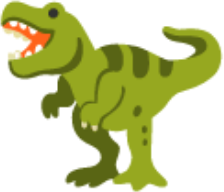
\includegraphics[height=2ex]{figuras/dino.png}}}
\renewcommand{\slateAuthor}{\textbf{Grupo 3}\\[1pt]\small Alvaro García \textperiodcentered\ Marcelin\dino\ Maita \textperiodcentered\ Diego Quispe \textperiodcentered\ Brigitte Rojas \textperiodcentered\ Sofía Salazar}
\renewcommand{\slateAdvisor}{Profesor: PhD.\ Rensso Mora Colque}
\renewcommand{\slateAffiliate}{Computer Vision \textperiodcentered\ Universidad de Ingeniería y Tecnología (UTEC)}
\renewcommand{\slateDate}{\small Lima, noviembre de 2026}

% ---- piezas con argumentos (en el preámbulo: beamer lee el cuerpo de un frame como argumento)
% una lección: \leccion{cifra}{afirmación}
\newcommand{\leccion}[2]{%
  \begin{tabular}{@{}p{32mm}@{\hspace{3mm}}p{\dimexpr\textwidth-35mm\relax}@{}}
    \leavevmode{\color{cAcc}\fontsize{16}{18}\selectfont #1} &
    \hyphenpenalty=10000\raggedright\leavevmode{\small #2\par}
  \end{tabular}\par\vspace{3.2mm}}
% un gesto de la Tarea B: \gesto{archivo}{acción}
\newcommand{\gesto}[2]{%
  \begin{minipage}[t]{0.322\linewidth}\centering
    \includegraphics[width=\linewidth]{figuras/gen/gesto_#1.jpg}\\[0.6mm]
    {\footnotesize\bfseries\color{cInk}#2}
  \end{minipage}}
% una decisión de diseño: \decision{icono}{decisión}{ganamos}{costo}
\newcommand{\decision}[4]{%
  \begin{minipage}[t]{0.48\textwidth}
    \begin{tabular}{@{}p{9mm}@{}p{\dimexpr\linewidth-9mm\relax}@{}}
      \leavevmode{\color{cAcc}\Large #1} &
      \raggedright\leavevmode{\small\bfseries #2\par}\vspace{0.8mm}
      {\footnotesize\color{cFila}\faPlus\ \color{cInk}#3\par}\vspace{0.4mm}
      {\footnotesize\color{cSrc}\faMinus\ \color{cInk}#4\par}
    \end{tabular}
  \end{minipage}}
% una fase de la línea de tiempo: \fase{y}{desde}{hasta}{color}{texto}  (x en s, 0.65 mm por segundo)
\newcommand{\fase}[5]{%
  \fill[#4] (#2*0.65,#1) rectangle (#3*0.65,#1+6);
  \node[font=\fontsize{6.5}{7.5}\selectfont\bfseries, text=white] at ({(#2+#3)/2*0.65},#1+3) {#5};}
% gráfico de barras horizontales con etiquetas a la izquierda y el valor al final de la barra
\pgfplotsset{barras/.style={sobrio, xbar, point meta=x, bar width=6pt, bar shift=0pt, y dir=reverse,
    axis x line=none, axis y line*=left, y axis line style={draw=none}, ytick style={draw=none},
    ytick=data, yticklabel style={font=\fontsize{7}{8}\selectfont, text=cInk, align=right},
    scale only axis, enlarge y limits={abs=0.6},
    nodes near coords, nodes near coords style={font=\fontsize{7}{8}\selectfont, text=cInk}}}

% generado por scripts/figuras.py: tubo:3, pose (0.9, 0.0, 0.0)
% \lidarpuntos{tamano de cada punto}: el scan (720 rayos, < 3 m) en el marco del robot (x adelante)
\newcommand{\lidarpuntos}[1]{\path plot[only marks, mark=*, mark size=#1, mark options={fill=cInk!85, draw=none}] coordinates {(-1.35,-0) (-1.35,-0.012) (-1.35,-0.024) (-1.35,-0.035) (-1.35,-0.047) (-1.35,-0.059) (-1.35,-0.071) (-1.35,-0.083) (-1.35,-0.094) (-1.35,-0.106) (-1.35,-0.118) (-1.35,-0.13) (-1.35,-0.142) (-1.35,-0.154) (-1.35,-0.166) (-1.35,-0.178) (-1.35,-0.19) (-1.35,-0.202) (-1.35,-0.214) (-1.35,-0.226) (-1.35,-0.238) (-1.35,-0.25) (-1.35,-0.262) (-1.35,-0.275) (-1.35,-0.287) (-1.35,-0.299) (-1.35,-0.312) (-1.35,-0.324) (-1.35,-0.337) (-1.35,-0.349) (-1.35,-0.362) (-1.35,-0.374) (-1.35,-0.387) (-1.35,-0.4) (-1.35,-0.413) (-1.35,-0.426) (-1.35,-0.439) (-1.345,-0.45) (-1.307,-0.45) (-1.271,-0.45) (-1.236,-0.45) (-1.204,-0.45) (-1.172,-0.45) (-1.142,-0.45) (-1.114,-0.45) (-1.086,-0.45) (-1.06,-0.45) (-1.035,-0.45) (-1.011,-0.45) (-0.987,-0.45) (-0.965,-0.45) (-0.943,-0.45) (-0.923,-0.45) (-0.903,-0.45) (-0.883,-0.45) (-0.864,-0.45) (-0.846,-0.45) (-0.829,-0.45) (-0.812,-0.45) (-0.795,-0.45) (-0.779,-0.45) (-0.764,-0.45) (-0.749,-0.45) (-0.734,-0.45) (-0.72,-0.45) (-0.706,-0.45) (-0.693,-0.45) (-0.68,-0.45) (-0.667,-0.45) (-0.655,-0.45) (-0.643,-0.45) (-0.631,-0.45) (-0.619,-0.45) (-0.608,-0.45) (-0.597,-0.45) (-0.586,-0.45) (-0.576,-0.45) (-0.566,-0.45) (-0.556,-0.45) (-0.546,-0.45) (-0.536,-0.45) (-0.527,-0.45) (-0.518,-0.45) (-0.509,-0.45) (-0.5,-0.45) (-0.491,-0.45) (-0.483,-0.45) (-0.474,-0.45) (-0.466,-0.45) (-0.458,-0.45) (-0.45,-0.45) (-0.442,-0.45) (-0.435,-0.45) (-0.427,-0.45) (-0.42,-0.45) (-0.412,-0.45) (-0.405,-0.45) (-0.398,-0.45) (-0.391,-0.45) (-0.384,-0.45) (-0.378,-0.45) (-0.371,-0.45) (-0.364,-0.45) (-0.358,-0.45) (-0.352,-0.45) (-0.345,-0.45) (-0.339,-0.45) (-0.333,-0.45) (-0.327,-0.45) (-0.321,-0.45) (-0.315,-0.45) (-0.309,-0.45) (-0.304,-0.45) (-0.298,-0.45) (-0.292,-0.45) (-0.287,-0.45) (-0.281,-0.45) (-0.276,-0.45) (-0.27,-0.45) (-0.265,-0.45) (-0.26,-0.45) (-0.255,-0.45) (-0.249,-0.45) (-0.244,-0.45) (-0.239,-0.45) (-0.234,-0.45) (-0.229,-0.45) (-0.224,-0.45) (-0.219,-0.45) (-0.215,-0.45) (-0.21,-0.45) (-0.205,-0.45) (-0.2,-0.45) (-0.196,-0.45) (-0.191,-0.45) (-0.186,-0.45) (-0.182,-0.45) (-0.177,-0.45) (-0.173,-0.45) (-0.168,-0.45) (-0.164,-0.45) (-0.159,-0.45) (-0.155,-0.45) (-0.151,-0.45) (-0.146,-0.45) (-0.142,-0.45) (-0.138,-0.45) (-0.133,-0.45) (-0.129,-0.45) (-0.125,-0.45) (-0.121,-0.45) (-0.116,-0.45) (-0.112,-0.45) (-0.108,-0.45) (-0.104,-0.45) (-0.1,-0.45) (-0.096,-0.45) (-0.092,-0.45) (-0.087,-0.45) (-0.083,-0.45) (-0.079,-0.45) (-0.075,-0.45) (-0.071,-0.45) (-0.067,-0.45) (-0.063,-0.45) (-0.059,-0.45) (-0.055,-0.45) (-0.051,-0.45) (-0.047,-0.45) (-0.043,-0.45) (-0.039,-0.45) (-0.035,-0.45) (-0.031,-0.45) (-0.028,-0.45) (-0.024,-0.45) (-0.02,-0.45) (-0.016,-0.45) (-0.012,-0.45) (-0.008,-0.45) (-0.004,-0.45) (0,-0.45) (0.004,-0.45) (0.008,-0.45) (0.012,-0.45) (0.016,-0.45) (0.02,-0.45) (0.024,-0.45) (0.028,-0.45) (0.031,-0.45) (0.035,-0.45) (0.039,-0.45) (0.043,-0.45) (0.047,-0.45) (0.051,-0.45) (0.055,-0.45) (0.059,-0.45) (0.063,-0.45) (0.067,-0.45) (0.071,-0.45) (0.075,-0.45) (0.079,-0.45) (0.083,-0.45) (0.087,-0.45) (0.092,-0.45) (0.096,-0.45) (0.1,-0.45) (0.104,-0.45) (0.108,-0.45) (0.112,-0.45) (0.116,-0.45) (0.121,-0.45) (0.125,-0.45) (0.129,-0.45) (0.133,-0.45) (0.138,-0.45) (0.142,-0.45) (0.146,-0.45) (0.151,-0.45) (0.155,-0.45) (0.159,-0.45) (0.164,-0.45) (0.168,-0.45) (0.173,-0.45) (0.177,-0.45) (0.182,-0.45) (0.186,-0.45) (0.191,-0.45) (0.196,-0.45) (0.2,-0.45) (0.205,-0.45) (0.21,-0.45) (0.215,-0.45) (0.219,-0.45) (0.224,-0.45) (0.229,-0.45) (0.234,-0.45) (0.239,-0.45) (0.244,-0.45) (0.249,-0.45) (0.255,-0.45) (0.26,-0.45) (0.265,-0.45) (0.27,-0.45) (0.276,-0.45) (0.281,-0.45) (0.287,-0.45) (0.292,-0.45) (0.298,-0.45) (0.304,-0.45) (0.309,-0.45) (0.315,-0.45) (0.321,-0.45) (0.327,-0.45) (0.333,-0.45) (0.339,-0.45) (0.345,-0.45) (0.352,-0.45) (0.358,-0.45) (0.364,-0.45) (0.371,-0.45) (0.378,-0.45) (0.384,-0.45) (0.391,-0.45) (0.398,-0.45) (0.405,-0.45) (0.412,-0.45) (0.42,-0.45) (0.427,-0.45) (0.435,-0.45) (0.442,-0.45) (0.45,-0.45) (0.458,-0.45) (0.466,-0.45) (0.474,-0.45) (0.483,-0.45) (0.491,-0.45) (0.5,-0.45) (0.509,-0.45) (0.518,-0.45) (0.527,-0.45) (0.536,-0.45) (0.546,-0.45) (0.556,-0.45) (0.566,-0.45) (0.576,-0.45) (0.586,-0.45) (0.597,-0.45) (0.608,-0.45) (0.619,-0.45) (0.631,-0.45) (0.643,-0.45) (0.655,-0.45) (0.667,-0.45) (0.68,-0.45) (0.693,-0.45) (0.706,-0.45) (0.72,-0.45) (0.734,-0.45) (0.749,-0.45) (0.764,-0.45) (0.779,-0.45) (0.795,-0.45) (0.812,-0.45) (0.829,-0.45) (0.846,-0.45) (0.864,-0.45) (0.883,-0.45) (0.903,-0.45) (0.923,-0.45) (0.943,-0.45) (0.965,-0.45) (0.987,-0.45) (1.011,-0.45) (1.035,-0.45) (1.95,-0.828) (1.95,-0.808) (1.95,-0.788) (1.95,-0.768) (1.95,-0.749) (1.95,-0.729) (1.95,-0.71) (1.95,-0.691) (1.95,-0.671) (1.95,-0.652) (1.95,-0.634) (1.95,-0.615) (1.95,-0.596) (1.95,-0.578) (1.95,-0.559) (1.95,-0.541) (1.95,-0.523) (1.95,-0.504) (1.95,-0.486) (1.95,-0.468) (1.95,-0.45) (1.95,-0.432) (1.95,-0.414) (1.95,-0.397) (1.95,-0.379) (1.95,-0.361) (1.95,-0.344) (1.95,-0.326) (1.95,-0.309) (1.95,-0.291) (1.95,-0.274) (1.95,-0.257) (1.95,-0.239) (1.95,-0.222) (1.95,-0.205) (1.95,-0.188) (1.95,-0.171) (1.95,-0.153) (1.95,-0.136) (1.95,-0.119) (1.95,-0.102) (1.95,-0.085) (1.95,-0.068) (1.95,-0.051) (1.95,-0.034) (1.95,-0.017) (1.95,0) (1.95,0.017) (1.95,0.034) (1.95,0.051) (1.95,0.068) (1.95,0.085) (1.95,0.102) (1.95,0.119) (1.95,0.136) (1.95,0.153) (1.95,0.171) (1.95,0.188) (1.95,0.205) (1.95,0.222) (1.95,0.239) (1.95,0.257) (1.95,0.274) (1.95,0.291) (0.947,0.15) (0.896,0.15) (0.851,0.15) (0.809,0.15) (0.772,0.15) (0.75,0.153) (0.73,0.155) (0.727,0.161) (0.727,0.168) (0.727,0.175) (0.727,0.181) (0.387,0.1) (0.373,0.1) (0.361,0.1) (0.349,0.1) (0.338,0.1) (0.327,0.1) (0.317,0.1) (0.308,0.1) (0.299,0.1) (0.29,0.1) (0.282,0.1) (0.275,0.1) (0.267,0.1) (0.261,0.1) (0.254,0.1) (0.248,0.1) (0.241,0.1) (0.236,0.1) (0.23,0.1) (0.225,0.1) (0.219,0.1) (0.214,0.1) (0.21,0.1) (0.205,0.1) (0.201,0.1) (0.196,0.1) (0.192,0.1) (0.188,0.1) (0.184,0.1) (0.18,0.1) (0.177,0.1) (0.173,0.1) (0.17,0.1) (0.166,0.1) (0.163,0.1) (0.16,0.1) (0.157,0.1) (0.154,0.1) (0.151,0.1) (0.148,0.1) (0.146,0.1) (0.143,0.1) (0.14,0.1) (0.138,0.1) (0.135,0.1) (0.133,0.1) (0.13,0.1) (0.128,0.1) (0.126,0.1) (0.123,0.1) (0.121,0.1) (0.119,0.1) (0.117,0.1) (0.115,0.1) (0.113,0.1) (0.111,0.1) (0.109,0.1) (0.107,0.1) (0.105,0.1) (0.104,0.1) (0.102,0.1) (0.1,0.1) (0.098,0.1) (0.097,0.1) (0.095,0.1) (0.093,0.1) (0.092,0.1) (0.09,0.1) (0.088,0.1) (0.087,0.1) (0.085,0.1) (0.084,0.1) (0.082,0.1) (0.081,0.1) (0.08,0.1) (0.078,0.1) (0.077,0.1) (0.075,0.1) (0.074,0.1) (0.073,0.1) (0.071,0.1) (0.07,0.1) (0.069,0.1) (0.067,0.1) (0.066,0.1) (0.065,0.1) (0.064,0.1) (0.062,0.1) (0.061,0.1) (0.06,0.1) (0.059,0.1) (0.058,0.1) (0.057,0.1) (0.055,0.1) (0.054,0.1) (0.053,0.1) (0.052,0.1) (0.051,0.1) (0.05,0.1) (0.05,0.103) (0.049,0.103) (0.048,0.103) (0.047,0.103) (0.046,0.103) (0.045,0.103) (0.044,0.103) (0.043,0.103) (0.042,0.103) (0.04,0.103) (0.039,0.103) (0.039,0.105) (0.039,0.108) (0.039,0.111) (0.039,0.114) (0.039,0.117) (0.039,0.121) (0.039,0.124) (0.039,0.128) (0.039,0.132) (0.039,0.137) (0.039,0.141) (0.039,0.146) (0.039,0.152) (0.039,0.157) (0.039,0.163) (0.039,0.17) (0.039,0.177) (0.039,0.184) (0.039,0.193) (0.039,0.202) (0.039,0.211) (0.039,0.222) (0.039,0.234) (0.039,0.247) (0.039,0.262) (0.039,0.279) (0.039,0.298) (0.039,0.319) (0.039,0.344) (0.039,0.373) (0.039,0.407) (0.039,0.448) (0.035,0.45) (0.031,0.45) (0.028,0.45) (0.024,0.45) (0.02,0.45) (0.016,0.45) (0.012,0.45) (0.008,0.45) (0.004,0.45) (0,0.45) (-0.004,0.45) (-0.008,0.45) (-0.012,0.45) (-0.016,0.45) (-0.02,0.45) (-0.024,0.45) (-0.028,0.45) (-0.031,0.45) (-0.035,0.45) (-0.039,0.45) (-0.043,0.45) (-0.047,0.45) (-0.051,0.45) (-0.055,0.45) (-0.059,0.45) (-0.063,0.45) (-0.067,0.45) (-0.071,0.45) (-0.075,0.45) (-0.079,0.45) (-0.083,0.45) (-0.087,0.45) (-0.092,0.45) (-0.096,0.45) (-0.1,0.45) (-0.104,0.45) (-0.108,0.45) (-0.112,0.45) (-0.116,0.45) (-0.121,0.45) (-0.125,0.45) (-0.129,0.45) (-0.133,0.45) (-0.138,0.45) (-0.142,0.45) (-0.146,0.45) (-0.151,0.45) (-0.155,0.45) (-0.159,0.45) (-0.164,0.45) (-0.168,0.45) (-0.173,0.45) (-0.177,0.45) (-0.182,0.45) (-0.186,0.45) (-0.191,0.45) (-0.196,0.45) (-0.2,0.45) (-0.205,0.45) (-0.21,0.45) (-0.215,0.45) (-0.219,0.45) (-0.224,0.45) (-0.229,0.45) (-0.234,0.45) (-0.239,0.45) (-0.244,0.45) (-0.249,0.45) (-0.255,0.45) (-0.26,0.45) (-0.265,0.45) (-0.27,0.45) (-0.276,0.45) (-0.281,0.45) (-0.287,0.45) (-0.292,0.45) (-0.298,0.45) (-0.304,0.45) (-0.309,0.45) (-0.315,0.45) (-0.321,0.45) (-0.327,0.45) (-0.333,0.45) (-0.339,0.45) (-0.345,0.45) (-0.352,0.45) (-0.358,0.45) (-0.364,0.45) (-0.371,0.45) (-0.378,0.45) (-0.384,0.45) (-0.391,0.45) (-0.398,0.45) (-0.405,0.45) (-0.412,0.45) (-0.42,0.45) (-0.427,0.45) (-0.435,0.45) (-0.442,0.45) (-0.45,0.45) (-0.458,0.45) (-0.466,0.45) (-0.474,0.45) (-0.483,0.45) (-0.491,0.45) (-0.5,0.45) (-0.509,0.45) (-0.518,0.45) (-0.527,0.45) (-0.536,0.45) (-0.546,0.45) (-0.556,0.45) (-0.566,0.45) (-0.576,0.45) (-0.586,0.45) (-0.597,0.45) (-0.608,0.45) (-0.619,0.45) (-0.631,0.45) (-0.643,0.45) (-0.655,0.45) (-0.667,0.45) (-0.68,0.45) (-0.693,0.45) (-0.706,0.45) (-0.72,0.45) (-0.734,0.45) (-0.749,0.45) (-0.764,0.45) (-0.779,0.45) (-0.795,0.45) (-0.812,0.45) (-0.829,0.45) (-0.846,0.45) (-0.864,0.45) (-0.883,0.45) (-0.903,0.45) (-0.923,0.45) (-0.943,0.45) (-0.965,0.45) (-0.987,0.45) (-1.011,0.45) (-1.035,0.45) (-1.06,0.45) (-1.086,0.45) (-1.114,0.45) (-1.142,0.45) (-1.172,0.45) (-1.204,0.45) (-1.236,0.45) (-1.271,0.45) (-1.307,0.45) (-1.345,0.45) (-1.35,0.439) (-1.35,0.426) (-1.35,0.413) (-1.35,0.4) (-1.35,0.387) (-1.35,0.374) (-1.35,0.362) (-1.35,0.349) (-1.35,0.337) (-1.35,0.324) (-1.35,0.312) (-1.35,0.299) (-1.35,0.287) (-1.35,0.275) (-1.35,0.262) (-1.35,0.25) (-1.35,0.238) (-1.35,0.226) (-1.35,0.214) (-1.35,0.202) (-1.35,0.19) (-1.35,0.178) (-1.35,0.166) (-1.35,0.154) (-1.35,0.142) (-1.35,0.13) (-1.35,0.118) (-1.35,0.106) (-1.35,0.094) (-1.35,0.083) (-1.35,0.071) (-1.35,0.059) (-1.35,0.047) (-1.35,0.035) (-1.35,0.024) (-1.35,0.012)};}
   % \lidarpuntos: el scan del LiDAR en el primer pasillo (diapositiva 3)

\begin{document}

% =============================================================================
% 1 · PORTADA
% =============================================================================
{\setbeamertemplate{headline}{}\setbeamertemplate{footline}{}
\begin{frame}[plain]
  \slatetitlepage
\end{frame}}

% =============================================================================
\section{Reto}
% =============================================================================

% 2 · el reto y la arquitectura ------------------------------------------------
\begin{frame}{El reto y nuestra arquitectura}
  \begin{columns}[c,onlytextwidth]
    \begin{column}{0.43\textwidth}\centering
      \begin{tikzpicture}[x=14mm, y=14mm]
        % generado por scripts/figuras.py: mundo tubo:3 y la ruta verdadera de figuras/datos/tubo_traza.json
\draw[pared] (1.95,-2.8) -- (2.85,-2.8);
\draw[pared] (-0.45,-0.45) -- (1.95,-0.45);
\draw[pared] (0.95,0.1) -- (1.3,0.1);
\draw[pared] (1.65,0.15) -- (1.9,0.15);
\draw[pared] (-0.45,0.45) -- (0.95,0.45);
\draw[pared] (1.3,0.45) -- (1.65,0.45);
\draw[pared] (1.9,0.45) -- (2.85,0.45);
\draw[pared] (-0.45,-0.45) -- (-0.45,0.45);
\draw[pared] (0.95,0.1) -- (0.95,0.45);
\draw[pared] (1.3,0.1) -- (1.3,0.45);
\draw[pared] (1.65,0.15) -- (1.65,0.45);
\draw[pared] (1.9,0.15) -- (1.9,0.45);
\draw[pared] (1.95,-2.8) -- (1.95,-0.45);
\draw[pared] (2.85,-2.8) -- (2.85,0.45);
\draw[pared] (0.939,0.103) -- (1.286,0.103);
\draw[pared] (1.286,0.103) -- (1.286,0.45);
\draw[pared] (1.286,0.45) -- (0.939,0.45);
\draw[pared] (0.939,0.45) -- (0.939,0.103);
\draw[pared] (1.627,0.155) -- (1.922,0.155);
\draw[pared] (1.922,0.155) -- (1.922,0.45);
\draw[pared] (1.922,0.45) -- (1.627,0.45);
\draw[pared] (1.627,0.45) -- (1.627,0.155);
\node[senal] (senal) at (2.846,-0.054) {};
\node[bandera] (bandera) at (2.366,-2.796) {};
\node[buscada] at (2.85,-0.991) {};
\node[foto] at (1.95,-1.01) {};
\node[foto] at (1.95,-1.54) {};
\node[foto] at (2.85,-2.028) {};
\draw[tIda] (-0.098,-0) -- (-0.033,-0.002) -- (0.057,-0.005) -- (0.147,-0.007) -- (0.237,-0.011) -- (0.327,-0.019) -- (0.416,-0.033) -- (0.504,-0.049) -- (0.593,-0.065) -- (0.682,-0.081) -- (0.77,-0.097) -- (0.859,-0.113) -- (0.947,-0.129) -- (1.036,-0.144) -- (1.125,-0.153) -- (1.215,-0.157) -- (1.305,-0.159) -- (1.395,-0.161) -- (1.485,-0.163) -- (1.575,-0.164) -- (1.665,-0.166) -- (1.755,-0.168) -- (1.845,-0.17) -- (1.935,-0.172) -- (2.025,-0.173) -- (2.115,-0.175) -- (2.203,-0.177) -- (2.289,-0.168) -- (2.35,-0.151) -- (2.401,-0.146) -- (2.433,-0.158) -- (2.452,-0.178) -- (2.472,-0.216) -- (2.496,-0.288) -- (2.513,-0.377) -- (2.523,-0.466) -- (2.53,-0.556) -- (2.536,-0.646) -- (2.543,-0.736) -- (2.545,-0.765);
\draw[tFila] (2.545,-0.765) -- (2.547,-0.84) -- (2.546,-0.915) -- (2.542,-0.99) -- (2.538,-1.065) -- (2.534,-1.14) -- (2.531,-1.215) -- (2.527,-1.29) -- (2.523,-1.365) -- (2.52,-1.44) -- (2.516,-1.515) -- (2.512,-1.589) -- (2.507,-1.664) -- (2.501,-1.739) -- (2.494,-1.814) -- (2.483,-1.888) -- (2.468,-1.961) -- (2.456,-2.01) -- (2.456,-2.01) -- (2.456,-2.01) -- (2.456,-2.01) -- (2.456,-2.01) -- (2.456,-2.01) -- (2.456,-2.01) -- (2.456,-2.01) -- (2.456,-2.01) -- (2.456,-2.01) -- (2.456,-2.01) -- (2.456,-2.01) -- (2.456,-2.01) -- (2.456,-2.01) -- (2.456,-2.01) -- (2.456,-2.01) -- (2.456,-2.01) -- (2.456,-2.01) -- (2.456,-2.01) -- (2.456,-2.01) -- (2.456,-2.01) -- (2.456,-2.01) -- (2.456,-2.01) -- (2.456,-2.01) -- (2.456,-2.01) -- (2.456,-2.01) -- (2.456,-2.01) -- (2.456,-2.01) -- (2.456,-2.01) -- (2.456,-2.01) -- (2.456,-2.01) -- (2.456,-2.01) -- (2.456,-2.01) -- (2.456,-2.01) -- (2.456,-2.01) -- (2.456,-2.01) -- (2.456,-2.01) -- (2.456,-2.01) -- (2.456,-2.01) -- (2.456,-2.01) -- (2.456,-2.01) -- (2.456,-2.01) -- (2.456,-2.01) -- (2.456,-2.01) -- (2.456,-2.01) -- (2.456,-2.01) -- (2.456,-2.01) -- (2.456,-2.01) -- (2.456,-2.01) -- (2.456,-2.01) -- (2.456,-2.01) -- (2.456,-2.01) -- (2.456,-2.01) -- (2.456,-2.01) -- (2.456,-2.01) -- (2.456,-2.01) -- (2.456,-2.01) -- (2.456,-2.01) -- (2.456,-2.01) -- (2.456,-2.01) -- (2.456,-2.01) -- (2.456,-2.01) -- (2.456,-2.01) -- (2.456,-2.01) -- (2.456,-2.01) -- (2.456,-2.01) -- (2.456,-2.01) -- (2.456,-2.01) -- (2.456,-2.01) -- (2.456,-2.01) -- (2.456,-2.01) -- (2.456,-2.01) -- (2.456,-2.01) -- (2.456,-2.01) -- (2.456,-2.01) -- (2.456,-2.01) -- (2.456,-2.01) -- (2.456,-2.01) -- (2.442,-2.02) -- (2.414,-2.03) -- (2.389,-2.026) -- (2.372,-2.014) -- (2.36,-2) -- (2.352,-1.984) -- (2.349,-1.978);
\draw[tQr] (2.349,-1.978) -- (2.349,-1.978) -- (2.349,-1.978) -- (2.349,-1.978) -- (2.349,-1.978) -- (2.349,-1.978) -- (2.349,-1.978) -- (2.349,-1.978) -- (2.349,-1.978) -- (2.349,-1.978) -- (2.349,-1.978) -- (2.349,-1.978) -- (2.349,-1.978) -- (2.349,-1.978) -- (2.349,-1.978);
\draw[tFila] (2.349,-1.978) -- (2.37,-2.002) -- (2.394,-2.029) -- (2.417,-2.056) -- (2.436,-2.078) -- (2.414,-2.038) -- (2.388,-1.968) -- (2.373,-1.895) -- (2.363,-1.82) -- (2.359,-1.746) -- (2.356,-1.671) -- (2.354,-1.596) -- (2.352,-1.521) -- (2.352,-1.471) -- (2.355,-1.464) -- (2.384,-1.438) -- (2.421,-1.43) -- (2.449,-1.438) -- (2.465,-1.455) -- (2.484,-1.497) -- (2.501,-1.568) -- (2.501,-1.583) -- (2.501,-1.583) -- (2.501,-1.583) -- (2.501,-1.583) -- (2.501,-1.583) -- (2.501,-1.583) -- (2.501,-1.583) -- (2.501,-1.583) -- (2.494,-1.584) -- (2.441,-1.6) -- (2.404,-1.63) -- (2.373,-1.677) -- (2.344,-1.745) -- (2.325,-1.817) -- (2.313,-1.891) -- (2.306,-1.966) -- (2.302,-2.041) -- (2.299,-2.116) -- (2.296,-2.191) -- (2.295,-2.253) -- (2.296,-2.278) -- (2.296,-2.278) -- (2.296,-2.278) -- (2.296,-2.278) -- (2.296,-2.278) -- (2.296,-2.278) -- (2.296,-2.278) -- (2.296,-2.278) -- (2.299,-2.278) -- (2.354,-2.276) -- (2.396,-2.257) -- (2.424,-2.227) -- (2.447,-2.186) -- (2.448,-2.184) -- (2.448,-2.184) -- (2.448,-2.184) -- (2.448,-2.184) -- (2.448,-2.184) -- (2.448,-2.184) -- (2.448,-2.184) -- (2.448,-2.184) -- (2.448,-2.184) -- (2.417,-2.178) -- (2.385,-2.16) -- (2.36,-2.131) -- (2.335,-2.082) -- (2.313,-2.01) -- (2.3,-1.937) -- (2.291,-1.862) -- (2.287,-1.787) -- (2.288,-1.737) -- (2.288,-1.737) -- (2.288,-1.737) -- (2.288,-1.737) -- (2.288,-1.737) -- (2.288,-1.737) -- (2.288,-1.737) -- (2.288,-1.737) -- (2.288,-1.737) -- (2.323,-1.73) -- (2.371,-1.705) -- (2.406,-1.663) -- (2.437,-1.596) -- (2.456,-1.524) -- (2.466,-1.45) -- (2.468,-1.409) -- (2.469,-1.391) -- (2.469,-1.39);
\draw[tQr] (2.469,-1.39) -- (2.469,-1.39) -- (2.469,-1.39) -- (2.469,-1.39) -- (2.469,-1.39) -- (2.469,-1.39) -- (2.469,-1.39) -- (2.469,-1.39) -- (2.469,-1.39) -- (2.469,-1.39) -- (2.469,-1.39) -- (2.469,-1.39) -- (2.469,-1.39) -- (2.469,-1.39) -- (2.469,-1.39) -- (2.469,-1.39) -- (2.469,-1.39) -- (2.469,-1.39);
\draw[tFila] (2.469,-1.39) -- (2.447,-1.413) -- (2.422,-1.439) -- (2.397,-1.465) -- (2.372,-1.49) -- (2.381,-1.477) -- (2.413,-1.41) -- (2.434,-1.338) -- (2.448,-1.265) -- (2.455,-1.215);
\draw[tVuelta] (2.455,-1.215) -- (2.464,-1.105) -- (2.47,-0.971) -- (2.477,-0.836) -- (2.483,-0.701) -- (2.468,-0.567) -- (2.421,-0.441) -- (2.346,-0.329) -- (2.266,-0.254) -- (2.216,-0.224) -- (2.162,-0.203) -- (2.071,-0.18) -- (1.939,-0.153) -- (1.812,-0.136) -- (1.742,-0.131) -- (1.623,-0.129) -- (1.488,-0.129) -- (1.353,-0.129) -- (1.218,-0.129) -- (1.083,-0.127) -- (0.948,-0.122) -- (0.813,-0.117) -- (0.678,-0.111) -- (0.544,-0.106) -- (0.409,-0.1) -- (0.303,-0.092) -- (0.214,-0.079) -- (0.142,-0.067) -- (0.096,-0.058) -- (0.096,-0.058) -- (0.096,-0.058) -- (0.096,-0.058) -- (0.096,-0.058);
\node[puntoA] (A) at (-0.1,0) {};
% caja: x -0.45..2.85  y -2.80..0.45

        \node[font=\small\bfseries, text=cInk, left=0.8mm of A] {A};
        \node[font=\small\bfseries, text=cInk, anchor=north] at (2.37,-2.95) {B};
        % leyenda, en el hueco de la L
        \begin{scope}[shift={(-0.35,-0.95)}, every node/.style={font=\fontsize{7}{8}\selectfont, anchor=west, text=cInk}]
          \draw[tIda] (0,0) -- (0.3,0);           \node at (0.35,0) {ida};
          \draw[tFila] (0,-0.3) -- (0.3,-0.3);     \node at (0.35,-0.3) {buscar en la meta};
          \draw[tQr] (0,-0.6) -- (0.3,-0.6);       \node at (0.35,-0.6) {leer el QR};
          \draw[tVuelta] (0,-0.9) -- (0.3,-0.9);   \node at (0.35,-0.9) {vuelta};
        \end{scope}
      \end{tikzpicture}
    \end{column}
    \begin{column}{0.55\textwidth}
      {\small Ir a la bandera, hallar a una persona entre 4 fotos, \textbf{leer su QR} y \textbf{volver a A}.\par}
      \vspace{4mm}
      \begin{tikzpicture}[x=1mm, y=1mm, every node/.append style={font=\footnotesize}]
        \node[grupo, minimum width=76mm, minimum height=28mm, anchor=north west] at (0,0) {};
        \node[font=\scriptsize\bfseries, text=cAcc, anchor=north west] at (1.5,-1) {\faRobot\ TurtleBot 4 (Raspberry Pi)};
        \node[caja, text width=22mm, font=\footnotesize] (se) at (14,-17) {LiDAR\\odometría\\cámara};
        \node[caja, text width=20mm, font=\footnotesize, draw=cAcc, line width=0.8pt] (pu) at (40,-17) {puente\\+ freno};
        \node[caja, text width=16mm, font=\footnotesize, draw=cIda, line width=0.8pt] (ta) at (65,-17) {\textbf{Tarea A}};
        \draw[ar] (se) -- (pu);
        \draw[ar, {Stealth[length=1.6mm]}-{Stealth[length=1.6mm]}] (pu) -- (ta);
        \node[grupo, minimum width=76mm, minimum height=14mm, anchor=north west] at (0,-38) {};
        \node[font=\scriptsize\bfseries, text=cAcc, anchor=north west] at (1.5,-39) {\faLaptop\ PC};
        \node[caja, text width=40mm, font=\footnotesize, draw=cFila, line width=0.8pt] (tb) at (40,-46) {\textbf{Tarea B}: gestos con la webcam};
        \draw[ar, {Stealth[length=1.6mm]}-{Stealth[length=1.6mm]}] (pu.south) -- node[lbl, right, font=\scriptsize]{UDP} (pu.south|-tb.north);
      \end{tikzpicture}\\[2mm]
    \end{column}
  \end{columns}
\end{frame}

% =============================================================================
\section{Sistema}
% =============================================================================

% 3 · sensores ---------------------------------------------------------------
\begin{frame}{Sensores}
  \begin{columns}[c,onlytextwidth]
    \begin{column}{0.6\textwidth}\centering
      \begin{tikzpicture}[x=33mm, y=33mm]
        \begin{scope}
          \clip (-0.45,-0.75) rectangle (2.02,0.45);
          \fill[cLight, opacity=0.16] (0.12,0) -- (1.95,{1.83*tan(21)}) -- (1.95,{-1.83*tan(21)}) -- cycle;
          \fill[cAcc, opacity=0.35] (0.17,-0.2) rectangle (0.28,0.2);
          \lidarpuntos{0.55pt}
          \draw[cInk, line width=0.6pt, fill=white] (0,0) circle (0.17);
          \draw[cInk, line width=0.8pt, -{Stealth[length=1.3mm]}] (0,0) -- (0.14,0);
        \end{scope}
        \node[senal] at (1.95,0.05) {};
        \node[font=\scriptsize, text=cAcc, anchor=east] (fr) at (-0.22,-0.32) {freno};
        \draw[cAcc, line width=0.3pt] (fr.east) -- (0.22,-0.05);
        \node[font=\scriptsize, text=cCelD, anchor=west] at (1.1,0.12) {cámara};
        \node[font=\scriptsize, text=cSrc] at (0.55,0.42) {caja};
        \node[font=\scriptsize, text=cSrc, anchor=north west] at (-0.45,0.62) {puntos: LiDAR};
      \end{tikzpicture}
    \end{column}
    \begin{column}{0.38\textwidth}
      \cifra{LiDAR}{720 distancias a 7\,Hz}
      \vspace{3mm}
      \cifra{Cámara}{OAK-D, $\sim$2 fotos/s}
      \vspace{3mm}
      \cifra{Webcam}{gestos (Tarea B)}
    \end{column}
  \end{columns}
  \vspace{3mm}
  {\footnotesize\color{cSrc}El freno vive en el robot: para a < 0.28\,m aunque falle la PC o el Wi-Fi.\par}
\end{frame}

% 4 · reconocimiento facial y QR ------------------------------------------------
\begin{frame}{Reconocimiento facial y QR}
  \centering
  \begin{tikzpicture}[x=1mm, y=1mm, l/.style={font=\scriptsize, text=cInk, align=center}]
    \node[img, anchor=west] (r) at (0,0) {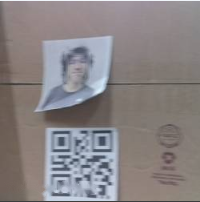
\includegraphics[height=24mm]{figuras/gen/robot_limpia.png}};
    \node[img, right=6mm of r] (y) {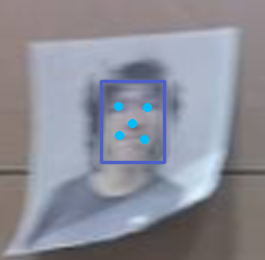
\includegraphics[height=24mm]{figuras/gen/cara_yunet.png}};
    \node[img, right=6mm of y] (a) {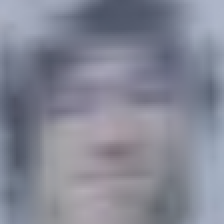
\includegraphics[height=15mm]{figuras/gen/cara_alineada.png}};
    \node[img, right=6mm of a] (e) {
\includegraphics[width=22mm, height=5mm]{figuras/gen/embedding.png}};
    \node[right=6mm of e, font=\large\bfseries, text=cAcc, align=center] (n) {Thiago\\[-0.5mm]Frias};
    \draw[ar] (r) -- (y); \draw[ar] (y) -- (a); \draw[ar] (a) -- (e); \draw[ar] (e) -- (n);
    \node[l, below=1.2mm of r] {cámara del robot};
    \node[l, below=1.2mm of y] {\textbf{YuNet}\\detecta};
    \node[l, below=5.5mm of a] {alinea};
    \node[l, below=1.5mm of e] {\textbf{ArcFace}\\512 números};
    \node[l, below=1mm of n] {la más parecida\\de 20 personas};
  \end{tikzpicture}

  \vspace{4mm}
  \begin{columns}[c,onlytextwidth]
    \begin{column}{0.44\textwidth}\centering
      \begin{tikzpicture}
        \begin{axis}[sobrio, width=46mm, height=26mm, scale only axis, xmin=12, xmax=50, ymin=70, ymax=101,
            xlabel={tamaño de la cara (px)}, ylabel={acierto (\%)}, xtick={14,24,32,48}, ytick={70,80,90,100},
            grid=major, legend pos=south east, legend cell align=left, mark size=1.3pt,
            xlabel style={yshift=1mm}, ylabel style={yshift=-2mm},
            legend style={font=\fontsize{6.5}{7.5}\selectfont}]
          \addplot[cMuted, mark=*] coordinates {(14,73.1) (18,85.4) (24,95.8) (32,99.0) (48,99.2)};
          \addlegendentry{1 foto}
          \addplot[cAcc, mark=*] coordinates {(14,82.6) (18,90.6) (24,99.1) (32,99.7) (48,100)};
          \addlegendentry{votando 4 fotos}
        \end{axis}
      \end{tikzpicture}
    \end{column}
    \begin{column}{0.28\textwidth}\centering
      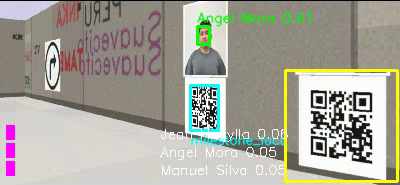
\includegraphics[width=\linewidth]{figuras/gen/sim_qr.png}
    \end{column}
    \begin{column}{0.26\textwidth}
      {\small\textbf{QR}: solo se acepta el que está \textbf{debajo de la cara buscada}.\par}

    \end{column}
  \end{columns}
\end{frame}

% =============================================================================
\section{Tarea A}
% =============================================================================

% 5 · navegación autónoma --------------------------------------------------------
\begin{frame}{Tarea A: navegación autónoma}
  \begin{columns}[c,onlytextwidth]
    \begin{column}{0.5\textwidth}\centering
      \begin{tikzpicture}[x=1mm, y=1mm, d/.style={font=\fontsize{6.5}{7.5}\selectfont, text=cSrc, align=center, anchor=north}]
        \node[est=cIda] (ida) at (0,0) {IDA};
        \node[est=cFila] (fila) at (24,0) {META};
        \node[est=cFila] (rec) at (50,0) {RECONOCER};
        \node[est=cFila] (qr) at (50,-24) {LEER QR};
        \node[est=cIda] (vol) at (24,-24) {VOLVER};
        \node[est=cIda] (fin) at (0,-24) {ANUNCIAR};
        \draw[ar] (ida) -- (fila); \draw[ar] (fila) -- (rec); \draw[ar] (rec) -- (qr);
        \draw[ar] (qr) -- (vol); \draw[ar] (vol) -- (fin);
        \node[d] at ([yshift=-1.2mm]ida.south) {sigue las\\flechas};
        \node[d] at ([yshift=-1.2mm]fila.south) {ve las\\4 fotos};
        \node[d, anchor=north east, align=right] at ([xshift=-1.5mm, yshift=-1.2mm]rec.south) {confirma\\de cerca};
        \node[d] at ([yshift=-1.2mm]vol.south) {turbo, Dijkstra\\e ICP};
      \end{tikzpicture}
    \end{column}
    \begin{column}{0.48\textwidth}\centering
      \begin{tikzpicture}[x=64mm, y=64mm]
        \begin{scope}
          \clip (-0.45,-0.2) rectangle (0.45,0.66);
          \begin{scope}[rotate=90]
            \draw[cInk!50, line width=0.5pt, fill=cPaper] (0,0) circle (0.175);
            % generado por scripts/figuras.py: tubo:3, pose (0.5, -0.1, 0.35), rumbo deseado -20 grados
\path plot[only marks, mark=*, mark size=0.55pt, mark options={fill=cInk!85, draw=none}] coordinates {(-1.011,-0) (-0.997,-0.009) (-0.974,-0.017) (-0.952,-0.025) (-0.932,-0.033) (-0.912,-0.04) (-0.893,-0.047) (-0.874,-0.053) (-0.857,-0.06) (-0.84,-0.066) (-0.823,-0.072) (-0.808,-0.078) (-0.793,-0.083) (-0.778,-0.089) (-0.764,-0.094) (-0.75,-0.099) (-0.737,-0.104) (-0.724,-0.108) (-0.712,-0.113) (-0.7,-0.117) (-0.688,-0.121) (-0.677,-0.125) (-0.666,-0.129) (-0.655,-0.133) (-0.645,-0.137) (-0.635,-0.141) (-0.625,-0.144) (-0.616,-0.148) (-0.606,-0.151) (-0.597,-0.155) (-0.589,-0.158) (-0.58,-0.161) (-0.572,-0.164) (-0.563,-0.167) (-0.555,-0.17) (-0.548,-0.173) (-0.54,-0.175) (-0.533,-0.178) (-0.525,-0.181) (-0.518,-0.183) (-0.511,-0.186) (-0.504,-0.189) (-0.498,-0.191) (-0.491,-0.193) (-0.484,-0.196) (-0.478,-0.198) (-0.472,-0.2) (-0.466,-0.203) (-0.46,-0.205) (-0.454,-0.207) (-0.448,-0.209) (-0.443,-0.211) (-0.437,-0.213) (-0.431,-0.215) (-0.426,-0.217) (-0.421,-0.219) (-0.415,-0.221) (-0.41,-0.223) (-0.405,-0.225) (-0.4,-0.226) (-0.395,-0.228) (-0.391,-0.23) (-0.386,-0.232) (-0.381,-0.233) (-0.376,-0.235) (-0.372,-0.237) (-0.367,-0.239) (-0.363,-0.24) (-0.358,-0.242) (-0.354,-0.243) (-0.35,-0.245) (-0.346,-0.246) (-0.341,-0.248) (-0.337,-0.25) (-0.333,-0.251) (-0.329,-0.252) (-0.325,-0.254) (-0.321,-0.255) (-0.317,-0.257) (-0.313,-0.258) (-0.309,-0.26) (-0.306,-0.261) (-0.302,-0.262) (-0.298,-0.264) (-0.294,-0.265) (-0.291,-0.266) (-0.287,-0.268) (-0.284,-0.269) (-0.28,-0.27) (-0.276,-0.272) (-0.273,-0.273) (-0.269,-0.274) (-0.266,-0.275) (-0.263,-0.277) (-0.259,-0.278) (-0.256,-0.279) (-0.252,-0.28) (-0.249,-0.282) (-0.246,-0.283) (-0.243,-0.284) (-0.239,-0.285) (-0.236,-0.286) (-0.233,-0.288) (-0.23,-0.289) (-0.227,-0.29) (-0.223,-0.291) (-0.22,-0.292) (-0.217,-0.293) (-0.214,-0.294) (-0.211,-0.296) (-0.208,-0.297) (-0.205,-0.298) (-0.202,-0.299) (-0.199,-0.3) (-0.196,-0.301) (-0.193,-0.302) (-0.19,-0.303) (-0.187,-0.304) (-0.184,-0.306) (-0.181,-0.307) (-0.178,-0.308) (-0.175,-0.309) (-0.172,-0.31) (-0.169,-0.311) (-0.166,-0.312) (-0.163,-0.313) (-0.16,-0.314) (-0.157,-0.315) (-0.154,-0.316) (-0.151,-0.317) (-0.148,-0.318) (-0.146,-0.319) (-0.143,-0.321) (-0.14,-0.322) (-0.137,-0.323) (-0.134,-0.324) (-0.131,-0.325) (-0.128,-0.326) (-0.125,-0.327) (-0.123,-0.328) (-0.12,-0.329) (-0.117,-0.33) (-0.114,-0.331) (-0.111,-0.332) (-0.108,-0.333) (-0.105,-0.334) (-0.102,-0.335) (-0.1,-0.336) (-0.097,-0.337) (-0.094,-0.338) (-0.091,-0.339) (-0.088,-0.34) (-0.085,-0.342) (-0.082,-0.343) (-0.079,-0.344) (-0.076,-0.345) (-0.073,-0.346) (-0.071,-0.347) (-0.068,-0.348) (-0.065,-0.349) (-0.062,-0.35) (-0.059,-0.351) (-0.056,-0.352) (-0.053,-0.353) (-0.05,-0.354) (-0.047,-0.356) (-0.044,-0.357) (-0.041,-0.358) (-0.038,-0.359) (-0.035,-0.36) (-0.032,-0.361) (-0.029,-0.362) (-0.025,-0.363) (-0.022,-0.364) (-0.019,-0.366) (-0.016,-0.367) (-0.013,-0.368) (-0.01,-0.369) (-0.006,-0.37) (-0.003,-0.371) (0,-0.373) (0.003,-0.374) (0.007,-0.375) (0.01,-0.376) (0.013,-0.377) (0.017,-0.379) (0.02,-0.38) (0.023,-0.381) (0.027,-0.382) (0.03,-0.384) (0.034,-0.385) (0.037,-0.386) (0.041,-0.387) (0.044,-0.389) (0.048,-0.39) (0.052,-0.391) (0.055,-0.393) (0.059,-0.394) (0.063,-0.395) (0.066,-0.397) (0.07,-0.398) (0.074,-0.4) (0.078,-0.401) (0.082,-0.402) (0.086,-0.404) (0.09,-0.405) (0.094,-0.407) (0.098,-0.408) (0.102,-0.41) (0.106,-0.411) (0.111,-0.413) (0.115,-0.415) (0.119,-0.416) (0.124,-0.418) (0.128,-0.419) (0.133,-0.421) (0.137,-0.423) (0.142,-0.424) (0.147,-0.426) (0.152,-0.428) (0.156,-0.43) (0.161,-0.431) (0.166,-0.433) (0.171,-0.435) (0.177,-0.437) (0.182,-0.439) (0.187,-0.441) (0.193,-0.443) (0.198,-0.445) (0.204,-0.447) (0.209,-0.449) (0.215,-0.451) (0.221,-0.453) (0.227,-0.455) (0.233,-0.458) (0.239,-0.46) (0.246,-0.462) (0.252,-0.465) (0.259,-0.467) (0.266,-0.47) (0.273,-0.472) (0.28,-0.475) (0.287,-0.477) (0.294,-0.48) (0.302,-0.483) (0.309,-0.485) (0.317,-0.488) (0.325,-0.491) (0.333,-0.494) (0.342,-0.497) (0.35,-0.501) (0.359,-0.504) (0.368,-0.507) (0.378,-0.51) (0.387,-0.514) (0.397,-0.518) (0.407,-0.521) (0.418,-0.525) (0.428,-0.529) (0.439,-0.533) (0.451,-0.537) (0.462,-0.541) (0.474,-0.546) (0.487,-0.55) (0.5,-0.555) (0.513,-0.56) (0.527,-0.565) (0.541,-0.57) (0.556,-0.575) (0.571,-0.581) (0.587,-0.587) (0.603,-0.593) (0.62,-0.599) (0.638,-0.606) (0.657,-0.612) (0.676,-0.619) (0.696,-0.627) (0.717,-0.634) (0.739,-0.642) (0.762,-0.651) (0.786,-0.659) (0.811,-0.669) (0.838,-0.678) (0.866,-0.689) (0.895,-0.699) (0.926,-0.711) (0.959,-0.723) (0.994,-0.735) (1.031,-0.749) (1.07,-0.763) (1.112,-0.778) (1.156,-0.795) (1.204,-0.812) (1.346,-0.225) (1.288,-0.204) (1.235,-0.185) (1.186,-0.167) (1.164,-0.153) (1.148,-0.141) (1.152,-0.131) (0.819,-0.086) (0.792,-0.076) (0.767,-0.067) (0.744,-0.059) (0.721,-0.05) (0.701,-0.043) (0.681,-0.036) (0.663,-0.029) (0.645,-0.023) (0.628,-0.016) (0.613,-0.011) (0.598,-0.005) (0.583,0) (0.57,0.005) (0.557,0.01) (0.544,0.014) (0.532,0.019) (0.521,0.023) (0.51,0.027) (0.5,0.031) (0.492,0.034) (0.486,0.038) (0.483,0.042) (0.485,0.047) (0.486,0.051) (0.488,0.056) (0.489,0.06) (0.491,0.065) (0.493,0.069) (0.495,0.074) (0.496,0.079) (0.498,0.083) (0.5,0.088) (0.501,0.093) (0.503,0.098) (0.505,0.103) (0.507,0.108) (0.509,0.113) (0.511,0.118) (0.512,0.123) (0.514,0.128) (0.516,0.134) (0.518,0.139) (0.52,0.144) (0.522,0.15) (0.524,0.155) (0.526,0.161) (0.528,0.167) (0.53,0.172) (0.533,0.178) (0.535,0.184) (0.537,0.19) (0.539,0.196) (0.541,0.202) (0.544,0.209) (0.546,0.215) (0.548,0.222) (0.551,0.228) (0.553,0.235) (0.556,0.242) (0.558,0.249) (0.561,0.256) (0.563,0.263) (0.566,0.27) (0.569,0.277) (0.572,0.285) (0.574,0.293) (0.577,0.3) (0.58,0.308) (0.583,0.317) (0.586,0.325) (0.589,0.333) (0.592,0.342) (0.596,0.351) (0.599,0.36) (0.599,0.367) (0.591,0.37) (0.584,0.372) (0.577,0.375) (0.57,0.377) (0.563,0.38) (0.556,0.382) (0.55,0.385) (0.543,0.387) (0.536,0.39) (0.53,0.392) (0.523,0.394) (0.517,0.397) (0.511,0.399) (0.505,0.401) (0.498,0.404) (0.492,0.406) (0.486,0.408) (0.48,0.41) (0.474,0.412) (0.468,0.414) (0.463,0.417) (0.457,0.419) (0.451,0.421) (0.446,0.423) (0.44,0.425) (0.434,0.427) (0.429,0.429) (0.423,0.431) (0.418,0.433) (0.413,0.435) (0.407,0.437) (0.402,0.439) (0.397,0.441) (0.392,0.443) (0.386,0.444) (0.381,0.446) (0.376,0.448) (0.371,0.45) (0.366,0.452) (0.361,0.454) (0.356,0.456) (0.351,0.457) (0.346,0.459) (0.341,0.461) (0.336,0.463) (0.331,0.465) (0.327,0.466) (0.322,0.468) (0.317,0.47) (0.312,0.472) (0.307,0.473) (0.303,0.475) (0.298,0.477) (0.293,0.478) (0.289,0.48) (0.284,0.482) (0.279,0.484) (0.275,0.485) (0.27,0.487) (0.265,0.489) (0.261,0.49) (0.256,0.492) (0.252,0.494) (0.247,0.495) (0.242,0.497) (0.238,0.499) (0.233,0.5) (0.229,0.502) (0.224,0.504) (0.22,0.505) (0.215,0.507) (0.211,0.509) (0.206,0.51) (0.202,0.512) (0.197,0.514) (0.193,0.515) (0.188,0.517) (0.184,0.518) (0.179,0.52) (0.175,0.522) (0.17,0.523) (0.166,0.525) (0.161,0.527) (0.157,0.528) (0.152,0.53) (0.147,0.532) (0.143,0.533) (0.138,0.535) (0.134,0.537) (0.129,0.538) (0.125,0.54) (0.12,0.542) (0.115,0.543) (0.111,0.545) (0.106,0.547) (0.102,0.548) (0.097,0.55) (0.092,0.552) (0.088,0.553) (0.083,0.555) (0.078,0.557) (0.074,0.559) (0.069,0.56) (0.064,0.562) (0.059,0.564) (0.054,0.566) (0.05,0.567) (0.045,0.569) (0.04,0.571) (0.035,0.573) (0.03,0.575) (0.025,0.576) (0.02,0.578) (0.015,0.58) (0.01,0.582) (0.005,0.584) (0,0.585) (-0.005,0.587) (-0.01,0.589) (-0.015,0.591) (-0.021,0.593) (-0.026,0.595) (-0.031,0.597) (-0.037,0.599) (-0.042,0.601) (-0.047,0.603) (-0.053,0.605) (-0.058,0.607) (-0.064,0.609) (-0.07,0.611) (-0.075,0.613) (-0.081,0.615) (-0.087,0.617) (-0.093,0.619) (-0.098,0.621) (-0.104,0.624) (-0.11,0.626) (-0.116,0.628) (-0.123,0.63) (-0.129,0.632) (-0.135,0.635) (-0.141,0.637) (-0.148,0.639) (-0.154,0.642) (-0.161,0.644) (-0.167,0.647) (-0.174,0.649) (-0.181,0.651) (-0.188,0.654) (-0.194,0.656) (-0.201,0.659) (-0.209,0.662) (-0.216,0.664) (-0.223,0.667) (-0.231,0.67) (-0.238,0.672) (-0.246,0.675) (-0.254,0.678) (-0.261,0.681) (-0.269,0.684) (-0.277,0.687) (-0.286,0.69) (-0.294,0.693) (-0.303,0.696) (-0.311,0.699) (-0.32,0.702) (-0.329,0.706) (-0.338,0.709) (-0.347,0.712) (-0.357,0.716) (-0.366,0.719) (-0.376,0.723) (-0.386,0.727) (-0.396,0.73) (-0.407,0.734) (-0.417,0.738) (-0.428,0.742) (-0.439,0.746) (-0.451,0.75) (-0.462,0.754) (-0.474,0.759) (-0.486,0.763) (-0.498,0.767) (-0.511,0.772) (-0.524,0.777) (-0.537,0.782) (-0.551,0.787) (-0.565,0.792) (-0.579,0.797) (-0.594,0.802) (-0.609,0.808) (-0.624,0.813) (-0.64,0.819) (-0.656,0.825) (-0.673,0.831) (-0.69,0.838) (-0.705,0.84) (-0.709,0.83) (-0.712,0.819) (-0.716,0.809) (-0.72,0.799) (-0.723,0.789) (-0.727,0.779) (-0.73,0.77) (-0.734,0.76) (-0.737,0.75) (-0.741,0.741) (-0.744,0.731) (-0.748,0.722) (-0.751,0.713) (-0.754,0.704) (-0.758,0.694) (-0.761,0.685) (-0.764,0.676) (-0.768,0.667) (-0.771,0.658) (-0.774,0.65) (-0.777,0.641) (-0.781,0.632) (-0.784,0.623) (-0.787,0.615) (-0.79,0.606) (-0.793,0.598) (-0.796,0.589) (-0.799,0.581) (-0.802,0.572) (-0.805,0.564) (-0.808,0.556) (-0.812,0.547) (-0.815,0.539) (-0.818,0.531) (-0.821,0.523) (-0.823,0.515) (-0.826,0.506) (-0.829,0.498) (-0.832,0.49) (-0.835,0.482) (-0.838,0.474) (-0.841,0.466) (-0.844,0.458) (-0.847,0.45) (-0.85,0.442) (-0.853,0.434) (-0.856,0.427) (-0.858,0.419) (-0.861,0.411) (-0.864,0.403) (-0.867,0.395) (-0.87,0.387) (-0.873,0.379) (-0.876,0.372) (-0.878,0.364) (-0.881,0.356) (-0.884,0.348) (-0.887,0.34) (-0.89,0.333) (-0.893,0.325) (-0.896,0.317) (-0.898,0.309) (-0.901,0.302) (-0.904,0.294) (-0.907,0.286) (-0.91,0.278) (-0.913,0.27) (-0.915,0.263) (-0.918,0.255) (-0.921,0.247) (-0.924,0.239) (-0.927,0.231) (-0.93,0.223) (-0.933,0.215) (-0.936,0.207) (-0.938,0.199) (-0.941,0.192) (-0.944,0.184) (-0.947,0.176) (-0.95,0.168) (-0.953,0.159) (-0.956,0.151) (-0.959,0.143) (-0.962,0.135) (-0.965,0.127) (-0.968,0.119) (-0.971,0.111) (-0.974,0.102) (-0.977,0.094) (-0.98,0.086) (-0.983,0.077) (-0.986,0.069) (-0.989,0.061) (-0.992,0.052) (-0.995,0.043) (-0.999,0.035) (-1.002,0.026) (-1.005,0.018) (-1.008,0.009)};
\draw[arcoMal] (0,0) -- (0.006,-0.001) -- (0.012,-0.002) -- (0.017,-0.005) -- (0.022,-0.008) -- (0.026,-0.013) -- (0.029,-0.018) -- (0.032,-0.023) -- (0.033,-0.029) -- (0.033,-0.035) -- (0.032,-0.041) -- (0.031,-0.047) -- (0.028,-0.052);
\draw[arcoMal] (0,0) -- (0.006,-0) -- (0.012,-0.002) -- (0.017,-0.004) -- (0.022,-0.007) -- (0.027,-0.011) -- (0.031,-0.016) -- (0.034,-0.021) -- (0.036,-0.027) -- (0.037,-0.033) -- (0.037,-0.039) -- (0.037,-0.045) -- (0.035,-0.05);
\draw[arcoMal] (0,0) -- (0.006,-0) -- (0.012,-0.002) -- (0.017,-0.004) -- (0.023,-0.007) -- (0.028,-0.01) -- (0.032,-0.014) -- (0.036,-0.019) -- (0.039,-0.024) -- (0.041,-0.03) -- (0.042,-0.036) -- (0.043,-0.042) -- (0.043,-0.048);
\draw[arcoMal] (0,0) -- (0.006,-0) -- (0.012,-0.001) -- (0.018,-0.003) -- (0.023,-0.006) -- (0.028,-0.009) -- (0.033,-0.012) -- (0.037,-0.017) -- (0.041,-0.021) -- (0.044,-0.026) -- (0.047,-0.032) -- (0.048,-0.038) -- (0.05,-0.043);
\draw[arcoMal] (0,0) -- (0.006,-0) -- (0.012,-0.001) -- (0.018,-0.003) -- (0.023,-0.005) -- (0.029,-0.007) -- (0.034,-0.01) -- (0.039,-0.014) -- (0.043,-0.018) -- (0.047,-0.023) -- (0.05,-0.028) -- (0.053,-0.033) -- (0.056,-0.038);
\draw[arcoOk] (0,0) -- (0.006,-0) -- (0.012,-0.001) -- (0.018,-0.002) -- (0.024,-0.004) -- (0.029,-0.006) -- (0.035,-0.008) -- (0.04,-0.011) -- (0.045,-0.015) -- (0.049,-0.019) -- (0.054,-0.023) -- (0.058,-0.027) -- (0.061,-0.032);
\draw[arcoOk] (0,0) -- (0.006,-0) -- (0.012,-0.001) -- (0.018,-0.002) -- (0.024,-0.003) -- (0.03,-0.004) -- (0.035,-0.006) -- (0.041,-0.009) -- (0.046,-0.011) -- (0.051,-0.014) -- (0.056,-0.017) -- (0.061,-0.021) -- (0.066,-0.025);
\draw[arcoOk] (0,0) -- (0.006,-0) -- (0.012,-0) -- (0.018,-0.001) -- (0.024,-0.002) -- (0.03,-0.003) -- (0.036,-0.004) -- (0.041,-0.006) -- (0.047,-0.008) -- (0.053,-0.01) -- (0.058,-0.012) -- (0.064,-0.014) -- (0.069,-0.017);
\draw[arcoOk] (0,0) -- (0.006,-0) -- (0.012,-0) -- (0.018,-0.001) -- (0.024,-0.001) -- (0.03,-0.001) -- (0.036,-0.002) -- (0.042,-0.003) -- (0.048,-0.004) -- (0.054,-0.005) -- (0.06,-0.006) -- (0.065,-0.007) -- (0.071,-0.009);
\draw[arcoOk] (0,0) -- (0.006,0) -- (0.012,0) -- (0.018,0) -- (0.024,0) -- (0.03,0) -- (0.036,0) -- (0.042,0) -- (0.048,0) -- (0.054,0) -- (0.06,0) -- (0.066,0) -- (0.072,0);
\draw[arcoOk] (0,0) -- (0.006,0) -- (0.012,0) -- (0.018,0.001) -- (0.024,0.001) -- (0.03,0.001) -- (0.036,0.002) -- (0.042,0.003) -- (0.048,0.004) -- (0.054,0.005) -- (0.06,0.006) -- (0.065,0.007) -- (0.071,0.009);
\draw[arcoOk] (0,0) -- (0.006,0) -- (0.012,0) -- (0.018,0.001) -- (0.024,0.002) -- (0.03,0.003) -- (0.036,0.004) -- (0.041,0.006) -- (0.047,0.008) -- (0.053,0.01) -- (0.058,0.012) -- (0.064,0.014) -- (0.069,0.017);
\draw[arcoOk] (0,0) -- (0.006,0) -- (0.012,0.001) -- (0.018,0.002) -- (0.024,0.003) -- (0.03,0.004) -- (0.035,0.006) -- (0.041,0.009) -- (0.046,0.011) -- (0.051,0.014) -- (0.056,0.017) -- (0.061,0.021) -- (0.066,0.025);
\draw[arcoOk] (0,0) -- (0.006,0) -- (0.012,0.001) -- (0.018,0.002) -- (0.024,0.004) -- (0.029,0.006) -- (0.035,0.008) -- (0.04,0.011) -- (0.045,0.015) -- (0.049,0.019) -- (0.054,0.023) -- (0.058,0.027) -- (0.061,0.032);
\draw[arcoOk] (0,0) -- (0.006,0) -- (0.012,0.001) -- (0.018,0.003) -- (0.023,0.005) -- (0.029,0.007) -- (0.034,0.01) -- (0.039,0.014) -- (0.043,0.018) -- (0.047,0.023) -- (0.05,0.028) -- (0.053,0.033) -- (0.056,0.038);
\draw[arcoOk] (0,0) -- (0.006,0) -- (0.012,0.001) -- (0.018,0.003) -- (0.023,0.006) -- (0.028,0.009) -- (0.033,0.012) -- (0.037,0.017) -- (0.041,0.021) -- (0.044,0.026) -- (0.047,0.032) -- (0.048,0.038) -- (0.05,0.043);
\draw[arcoOk] (0,0) -- (0.006,0) -- (0.012,0.002) -- (0.017,0.004) -- (0.023,0.007) -- (0.028,0.01) -- (0.032,0.014) -- (0.036,0.019) -- (0.039,0.024) -- (0.041,0.03) -- (0.042,0.036) -- (0.043,0.042) -- (0.043,0.048);
\draw[arcoOk] (0,0) -- (0.006,0) -- (0.012,0.002) -- (0.017,0.004) -- (0.022,0.007) -- (0.027,0.011) -- (0.031,0.016) -- (0.034,0.021) -- (0.036,0.027) -- (0.037,0.033) -- (0.037,0.039) -- (0.037,0.045) -- (0.035,0.05);
\draw[arcoOk] (0,0) -- (0.006,0.001) -- (0.012,0.002) -- (0.017,0.005) -- (0.022,0.008) -- (0.026,0.013) -- (0.029,0.018) -- (0.032,0.023) -- (0.033,0.029) -- (0.033,0.035) -- (0.032,0.041) -- (0.031,0.047) -- (0.028,0.052);
\draw[arcoMal] (0,0) -- (0.012,-0.001) -- (0.023,-0.004) -- (0.034,-0.009) -- (0.044,-0.017) -- (0.052,-0.025) -- (0.059,-0.035) -- (0.063,-0.046) -- (0.066,-0.058) -- (0.067,-0.07) -- (0.065,-0.082) -- (0.061,-0.093) -- (0.055,-0.104);
\draw[arcoMal] (0,0) -- (0.012,-0.001) -- (0.024,-0.004) -- (0.035,-0.008) -- (0.045,-0.015) -- (0.054,-0.023) -- (0.061,-0.032) -- (0.068,-0.042) -- (0.072,-0.053) -- (0.074,-0.065) -- (0.075,-0.077) -- (0.074,-0.089) -- (0.07,-0.101);
\draw[arcoMal] (0,0) -- (0.012,-0.001) -- (0.024,-0.003) -- (0.035,-0.007) -- (0.046,-0.013) -- (0.055,-0.02) -- (0.064,-0.029) -- (0.071,-0.038) -- (0.077,-0.048) -- (0.082,-0.06) -- (0.084,-0.071) -- (0.086,-0.083) -- (0.085,-0.095);
\draw[arcoMal] (0,0) -- (0.012,-0.001) -- (0.024,-0.003) -- (0.035,-0.006) -- (0.046,-0.011) -- (0.056,-0.017) -- (0.066,-0.025) -- (0.074,-0.033) -- (0.082,-0.043) -- (0.088,-0.053) -- (0.093,-0.064) -- (0.097,-0.075) -- (0.099,-0.087);
\draw[arcoMal] (0,0) -- (0.012,-0.001) -- (0.024,-0.002) -- (0.035,-0.005) -- (0.047,-0.009) -- (0.058,-0.015) -- (0.068,-0.021) -- (0.077,-0.028) -- (0.086,-0.036) -- (0.094,-0.045) -- (0.101,-0.055) -- (0.107,-0.066) -- (0.112,-0.077);
\draw[arcoMal] (0,0) -- (0.012,-0) -- (0.024,-0.002) -- (0.036,-0.004) -- (0.047,-0.008) -- (0.058,-0.012) -- (0.069,-0.017) -- (0.08,-0.023) -- (0.09,-0.03) -- (0.099,-0.037) -- (0.108,-0.045) -- (0.116,-0.054) -- (0.123,-0.064);
\draw[arcoOk] (0,0) -- (0.012,-0) -- (0.024,-0.001) -- (0.036,-0.003) -- (0.048,-0.006) -- (0.059,-0.009) -- (0.07,-0.013) -- (0.082,-0.017) -- (0.092,-0.023) -- (0.103,-0.028) -- (0.113,-0.035) -- (0.123,-0.042) -- (0.132,-0.05);
\draw[arcoOk] (0,0) -- (0.012,-0) -- (0.024,-0.001) -- (0.036,-0.002) -- (0.048,-0.004) -- (0.06,-0.006) -- (0.071,-0.009) -- (0.083,-0.012) -- (0.094,-0.015) -- (0.106,-0.019) -- (0.117,-0.024) -- (0.128,-0.029) -- (0.139,-0.034);
\draw[arcoOk] (0,0) -- (0.012,-0) -- (0.024,-0) -- (0.036,-0.001) -- (0.048,-0.002) -- (0.06,-0.003) -- (0.072,-0.004) -- (0.084,-0.006) -- (0.096,-0.008) -- (0.107,-0.01) -- (0.119,-0.012) -- (0.131,-0.014) -- (0.143,-0.017);
\draw[arcoOk] (0,0) -- (0.012,0) -- (0.024,0) -- (0.036,0) -- (0.048,0) -- (0.06,0) -- (0.072,0) -- (0.084,0) -- (0.096,0) -- (0.108,0) -- (0.12,0) -- (0.132,0) -- (0.144,0);
\draw[arcoOk] (0,0) -- (0.012,0) -- (0.024,0) -- (0.036,0.001) -- (0.048,0.002) -- (0.06,0.003) -- (0.072,0.004) -- (0.084,0.006) -- (0.096,0.008) -- (0.107,0.01) -- (0.119,0.012) -- (0.131,0.014) -- (0.143,0.017);
\draw[arcoOk] (0,0) -- (0.012,0) -- (0.024,0.001) -- (0.036,0.002) -- (0.048,0.004) -- (0.06,0.006) -- (0.071,0.009) -- (0.083,0.012) -- (0.094,0.015) -- (0.106,0.019) -- (0.117,0.024) -- (0.128,0.029) -- (0.139,0.034);
\draw[arcoOk] (0,0) -- (0.012,0) -- (0.024,0.001) -- (0.036,0.003) -- (0.048,0.006) -- (0.059,0.009) -- (0.07,0.013) -- (0.082,0.017) -- (0.092,0.023) -- (0.103,0.028) -- (0.113,0.035) -- (0.123,0.042) -- (0.132,0.05);
\draw[arcoOk] (0,0) -- (0.012,0) -- (0.024,0.002) -- (0.036,0.004) -- (0.047,0.008) -- (0.058,0.012) -- (0.069,0.017) -- (0.08,0.023) -- (0.09,0.03) -- (0.099,0.037) -- (0.108,0.045) -- (0.116,0.054) -- (0.123,0.064);
\draw[arcoOk] (0,0) -- (0.012,0.001) -- (0.024,0.002) -- (0.035,0.005) -- (0.047,0.009) -- (0.058,0.015) -- (0.068,0.021) -- (0.077,0.028) -- (0.086,0.036) -- (0.094,0.045) -- (0.101,0.055) -- (0.107,0.066) -- (0.112,0.077);
\draw[arcoOk] (0,0) -- (0.012,0.001) -- (0.024,0.003) -- (0.035,0.006) -- (0.046,0.011) -- (0.056,0.017) -- (0.066,0.025) -- (0.074,0.033) -- (0.082,0.043) -- (0.088,0.053) -- (0.093,0.064) -- (0.097,0.075) -- (0.099,0.087);
\draw[arcoOk] (0,0) -- (0.012,0.001) -- (0.024,0.003) -- (0.035,0.007) -- (0.046,0.013) -- (0.055,0.02) -- (0.064,0.029) -- (0.071,0.038) -- (0.077,0.048) -- (0.082,0.06) -- (0.084,0.071) -- (0.086,0.083) -- (0.085,0.095);
\draw[arcoOk] (0,0) -- (0.012,0.001) -- (0.024,0.004) -- (0.035,0.008) -- (0.045,0.015) -- (0.054,0.023) -- (0.061,0.032) -- (0.068,0.042) -- (0.072,0.053) -- (0.074,0.065) -- (0.075,0.077) -- (0.074,0.089) -- (0.07,0.101);
\draw[arcoOk] (0,0) -- (0.012,0.001) -- (0.023,0.004) -- (0.034,0.009) -- (0.044,0.017) -- (0.052,0.025) -- (0.059,0.035) -- (0.063,0.046) -- (0.066,0.058) -- (0.067,0.07) -- (0.065,0.082) -- (0.061,0.093) -- (0.055,0.104);
\draw[arcoMal] (0,0) -- (0.018,-0.002) -- (0.035,-0.006) -- (0.051,-0.014) -- (0.066,-0.025) -- (0.078,-0.038) -- (0.088,-0.053) -- (0.095,-0.069) -- (0.099,-0.087) -- (0.1,-0.105) -- (0.097,-0.123) -- (0.092,-0.14) -- (0.083,-0.156);
\draw[arcoMal] (0,0) -- (0.018,-0.001) -- (0.035,-0.006) -- (0.052,-0.013) -- (0.067,-0.022) -- (0.081,-0.034) -- (0.092,-0.048) -- (0.101,-0.063) -- (0.108,-0.08) -- (0.112,-0.098) -- (0.112,-0.116) -- (0.11,-0.134) -- (0.106,-0.151);
\draw[arcoMal] (0,0) -- (0.018,-0.001) -- (0.036,-0.005) -- (0.052,-0.011) -- (0.068,-0.02) -- (0.083,-0.03) -- (0.096,-0.043) -- (0.107,-0.057) -- (0.116,-0.073) -- (0.122,-0.089) -- (0.127,-0.107) -- (0.129,-0.125) -- (0.128,-0.143);
\draw[arcoMal] (0,0) -- (0.018,-0.001) -- (0.036,-0.004) -- (0.053,-0.01) -- (0.069,-0.017) -- (0.085,-0.026) -- (0.099,-0.037) -- (0.112,-0.05) -- (0.123,-0.064) -- (0.132,-0.079) -- (0.14,-0.096) -- (0.145,-0.113) -- (0.149,-0.13);
\draw[arcoMal] (0,0) -- (0.018,-0.001) -- (0.036,-0.004) -- (0.053,-0.008) -- (0.07,-0.014) -- (0.086,-0.022) -- (0.102,-0.031) -- (0.116,-0.042) -- (0.129,-0.055) -- (0.141,-0.068) -- (0.151,-0.083) -- (0.16,-0.098) -- (0.168,-0.115);
\draw[arcoMal] (0,0) -- (0.018,-0.001) -- (0.036,-0.003) -- (0.053,-0.006) -- (0.071,-0.011) -- (0.088,-0.018) -- (0.104,-0.025) -- (0.12,-0.034) -- (0.134,-0.045) -- (0.148,-0.056) -- (0.161,-0.068) -- (0.173,-0.082) -- (0.184,-0.096);
\draw[arcoOk] (0,0) -- (0.018,-0.001) -- (0.036,-0.002) -- (0.054,-0.005) -- (0.071,-0.009) -- (0.089,-0.013) -- (0.106,-0.019) -- (0.122,-0.026) -- (0.139,-0.034) -- (0.154,-0.043) -- (0.169,-0.052) -- (0.184,-0.063) -- (0.198,-0.074);
\draw[arcoMal] (0,0) -- (0.018,-0) -- (0.036,-0.001) -- (0.054,-0.003) -- (0.072,-0.006) -- (0.089,-0.009) -- (0.107,-0.013) -- (0.124,-0.018) -- (0.142,-0.023) -- (0.159,-0.029) -- (0.175,-0.036) -- (0.192,-0.043) -- (0.208,-0.051);
\draw[arcoMal] (0,0) -- (0.018,-0) -- (0.036,-0.001) -- (0.054,-0.002) -- (0.072,-0.003) -- (0.09,-0.004) -- (0.108,-0.006) -- (0.126,-0.009) -- (0.143,-0.011) -- (0.161,-0.015) -- (0.179,-0.018) -- (0.196,-0.022) -- (0.214,-0.026);
\draw[arcoMal] (0,0) -- (0.018,0) -- (0.036,0) -- (0.054,0) -- (0.072,0) -- (0.09,0) -- (0.108,0) -- (0.126,0) -- (0.144,0) -- (0.162,0) -- (0.18,0) -- (0.198,0) -- (0.216,0);
\draw[arcoMal] (0,0) -- (0.018,0) -- (0.036,0.001) -- (0.054,0.002) -- (0.072,0.003) -- (0.09,0.004) -- (0.108,0.006) -- (0.126,0.009) -- (0.143,0.011) -- (0.161,0.015) -- (0.179,0.018) -- (0.196,0.022) -- (0.214,0.026);
\draw[arcoMal] (0,0) -- (0.018,0) -- (0.036,0.001) -- (0.054,0.003) -- (0.072,0.006) -- (0.089,0.009) -- (0.107,0.013) -- (0.124,0.018) -- (0.142,0.023) -- (0.159,0.029) -- (0.175,0.036) -- (0.192,0.043) -- (0.208,0.051);
\draw[arcoMal] (0,0) -- (0.018,0.001) -- (0.036,0.002) -- (0.054,0.005) -- (0.071,0.009) -- (0.089,0.013) -- (0.106,0.019) -- (0.122,0.026) -- (0.139,0.034) -- (0.154,0.043) -- (0.169,0.052) -- (0.184,0.063) -- (0.198,0.074);
\draw[arcoMal] (0,0) -- (0.018,0.001) -- (0.036,0.003) -- (0.053,0.006) -- (0.071,0.011) -- (0.088,0.018) -- (0.104,0.025) -- (0.12,0.034) -- (0.134,0.045) -- (0.148,0.056) -- (0.161,0.068) -- (0.173,0.082) -- (0.184,0.096);
\draw[arcoOk] (0,0) -- (0.018,0.001) -- (0.036,0.004) -- (0.053,0.008) -- (0.07,0.014) -- (0.086,0.022) -- (0.102,0.031) -- (0.116,0.042) -- (0.129,0.055) -- (0.141,0.068) -- (0.151,0.083) -- (0.16,0.098) -- (0.168,0.115);
\draw[arcoOk] (0,0) -- (0.018,0.001) -- (0.036,0.004) -- (0.053,0.01) -- (0.069,0.017) -- (0.085,0.026) -- (0.099,0.037) -- (0.112,0.05) -- (0.123,0.064) -- (0.132,0.079) -- (0.14,0.096) -- (0.145,0.113) -- (0.149,0.13);
\draw[arcoOk] (0,0) -- (0.018,0.001) -- (0.036,0.005) -- (0.052,0.011) -- (0.068,0.02) -- (0.083,0.03) -- (0.096,0.043) -- (0.107,0.057) -- (0.116,0.073) -- (0.122,0.089) -- (0.127,0.107) -- (0.129,0.125) -- (0.128,0.143);
\draw[arcoOk] (0,0) -- (0.018,0.001) -- (0.035,0.006) -- (0.052,0.013) -- (0.067,0.022) -- (0.081,0.034) -- (0.092,0.048) -- (0.101,0.063) -- (0.108,0.08) -- (0.112,0.098) -- (0.112,0.116) -- (0.11,0.134) -- (0.106,0.151);
\draw[arcoOk] (0,0) -- (0.018,0.002) -- (0.035,0.006) -- (0.051,0.014) -- (0.066,0.025) -- (0.078,0.038) -- (0.088,0.053) -- (0.095,0.069) -- (0.099,0.087) -- (0.1,0.105) -- (0.097,0.123) -- (0.092,0.14) -- (0.083,0.156);
\draw[arcoMal] (0,0) -- (0.024,-0.002) -- (0.047,-0.009) -- (0.069,-0.019) -- (0.088,-0.033) -- (0.104,-0.05) -- (0.118,-0.07) -- (0.127,-0.093) -- (0.132,-0.116) -- (0.133,-0.14) -- (0.13,-0.164) -- (0.122,-0.186) -- (0.111,-0.207);
\draw[arcoMal] (0,0) -- (0.024,-0.002) -- (0.047,-0.008) -- (0.069,-0.017) -- (0.09,-0.03) -- (0.108,-0.045) -- (0.123,-0.064) -- (0.135,-0.085) -- (0.144,-0.107) -- (0.149,-0.13) -- (0.15,-0.154) -- (0.147,-0.178) -- (0.141,-0.201);
\draw[arcoMal] (0,0) -- (0.024,-0.002) -- (0.047,-0.007) -- (0.07,-0.015) -- (0.091,-0.026) -- (0.11,-0.04) -- (0.128,-0.057) -- (0.142,-0.076) -- (0.154,-0.097) -- (0.163,-0.119) -- (0.169,-0.142) -- (0.171,-0.166) -- (0.17,-0.19);
\draw[arcoMal] (0,0) -- (0.024,-0.001) -- (0.048,-0.006) -- (0.07,-0.013) -- (0.092,-0.023) -- (0.113,-0.035) -- (0.132,-0.05) -- (0.149,-0.067) -- (0.164,-0.085) -- (0.176,-0.106) -- (0.186,-0.128) -- (0.194,-0.15) -- (0.198,-0.174);
\draw[arcoMal] (0,0) -- (0.024,-0.001) -- (0.048,-0.005) -- (0.071,-0.011) -- (0.093,-0.019) -- (0.115,-0.029) -- (0.136,-0.042) -- (0.155,-0.056) -- (0.172,-0.073) -- (0.188,-0.091) -- (0.202,-0.11) -- (0.214,-0.131) -- (0.224,-0.153);
\draw[arcoMal] (0,0) -- (0.024,-0.001) -- (0.048,-0.004) -- (0.071,-0.009) -- (0.094,-0.015) -- (0.117,-0.024) -- (0.139,-0.034) -- (0.159,-0.046) -- (0.179,-0.059) -- (0.198,-0.074) -- (0.215,-0.091) -- (0.231,-0.109) -- (0.246,-0.128);
\draw[arcoMal] (0,0) -- (0.024,-0.001) -- (0.048,-0.003) -- (0.072,-0.006) -- (0.095,-0.011) -- (0.118,-0.018) -- (0.141,-0.026) -- (0.163,-0.035) -- (0.185,-0.045) -- (0.206,-0.057) -- (0.226,-0.07) -- (0.245,-0.084) -- (0.264,-0.099);
\draw[arcoMal] (0,0) -- (0.024,-0) -- (0.048,-0.002) -- (0.072,-0.004) -- (0.096,-0.008) -- (0.119,-0.012) -- (0.143,-0.017) -- (0.166,-0.023) -- (0.189,-0.03) -- (0.211,-0.038) -- (0.234,-0.047) -- (0.256,-0.057) -- (0.277,-0.068);
\draw[arcoMal] (0,0) -- (0.024,-0) -- (0.048,-0.001) -- (0.072,-0.002) -- (0.096,-0.004) -- (0.12,-0.006) -- (0.144,-0.009) -- (0.167,-0.012) -- (0.191,-0.015) -- (0.215,-0.019) -- (0.238,-0.024) -- (0.262,-0.029) -- (0.285,-0.034);
\draw[arcoMal] (0,0) -- (0.024,0) -- (0.048,0) -- (0.072,0) -- (0.096,0) -- (0.12,0) -- (0.144,0) -- (0.168,0) -- (0.192,0) -- (0.216,0) -- (0.24,0) -- (0.264,0) -- (0.288,0);
\draw[arcoMal] (0,0) -- (0.024,0) -- (0.048,0.001) -- (0.072,0.002) -- (0.096,0.004) -- (0.12,0.006) -- (0.144,0.009) -- (0.167,0.012) -- (0.191,0.015) -- (0.215,0.019) -- (0.238,0.024) -- (0.262,0.029) -- (0.285,0.034);
\draw[arcoMal] (0,0) -- (0.024,0) -- (0.048,0.002) -- (0.072,0.004) -- (0.096,0.008) -- (0.119,0.012) -- (0.143,0.017) -- (0.166,0.023) -- (0.189,0.03) -- (0.211,0.038) -- (0.234,0.047) -- (0.256,0.057) -- (0.277,0.068);
\draw[arcoMal] (0,0) -- (0.024,0.001) -- (0.048,0.003) -- (0.072,0.006) -- (0.095,0.011) -- (0.118,0.018) -- (0.141,0.026) -- (0.163,0.035) -- (0.185,0.045) -- (0.206,0.057) -- (0.226,0.07) -- (0.245,0.084) -- (0.264,0.099);
\draw[arcoMal] (0,0) -- (0.024,0.001) -- (0.048,0.004) -- (0.071,0.009) -- (0.094,0.015) -- (0.117,0.024) -- (0.139,0.034) -- (0.159,0.046) -- (0.179,0.059) -- (0.198,0.074) -- (0.215,0.091) -- (0.231,0.109) -- (0.246,0.128);
\draw[arcoMal] (0,0) -- (0.024,0.001) -- (0.048,0.005) -- (0.071,0.011) -- (0.093,0.019) -- (0.115,0.029) -- (0.136,0.042) -- (0.155,0.056) -- (0.172,0.073) -- (0.188,0.091) -- (0.202,0.11) -- (0.214,0.131) -- (0.224,0.153);
\draw[arcoMal] (0,0) -- (0.024,0.001) -- (0.048,0.006) -- (0.07,0.013) -- (0.092,0.023) -- (0.113,0.035) -- (0.132,0.05) -- (0.149,0.067) -- (0.164,0.085) -- (0.176,0.106) -- (0.186,0.128) -- (0.194,0.15) -- (0.198,0.174);
\draw[arcoMal] (0,0) -- (0.024,0.002) -- (0.047,0.007) -- (0.07,0.015) -- (0.091,0.026) -- (0.11,0.04) -- (0.128,0.057) -- (0.142,0.076) -- (0.154,0.097) -- (0.163,0.119) -- (0.169,0.142) -- (0.171,0.166) -- (0.17,0.19);
\draw[arcoMal] (0,0) -- (0.024,0.002) -- (0.047,0.008) -- (0.069,0.017) -- (0.09,0.03) -- (0.108,0.045) -- (0.123,0.064) -- (0.135,0.085) -- (0.144,0.107) -- (0.149,0.13) -- (0.15,0.154) -- (0.147,0.178) -- (0.141,0.201);
\draw[arcoMal] (0,0) -- (0.024,0.002) -- (0.047,0.009) -- (0.069,0.019) -- (0.088,0.033) -- (0.104,0.05) -- (0.118,0.07) -- (0.127,0.093) -- (0.132,0.116) -- (0.133,0.14) -- (0.13,0.164) -- (0.122,0.186) -- (0.111,0.207);
\draw[arcoMal] (0,0) -- (0.03,-0.003) -- (0.059,-0.011) -- (0.086,-0.024) -- (0.11,-0.041) -- (0.131,-0.063) -- (0.147,-0.088) -- (0.159,-0.116) -- (0.165,-0.145) -- (0.166,-0.175) -- (0.162,-0.205) -- (0.153,-0.233) -- (0.139,-0.259);
\draw[arcoMal] (0,0) -- (0.03,-0.002) -- (0.059,-0.01) -- (0.087,-0.021) -- (0.112,-0.037) -- (0.135,-0.057) -- (0.154,-0.08) -- (0.169,-0.106) -- (0.18,-0.134) -- (0.186,-0.163) -- (0.187,-0.193) -- (0.184,-0.223) -- (0.176,-0.252);
\draw[arcoMal] (0,0) -- (0.03,-0.002) -- (0.059,-0.008) -- (0.087,-0.019) -- (0.114,-0.033) -- (0.138,-0.05) -- (0.16,-0.071) -- (0.178,-0.095) -- (0.193,-0.121) -- (0.204,-0.149) -- (0.211,-0.178) -- (0.214,-0.208) -- (0.213,-0.238);
\draw[arcoMal] (0,0) -- (0.03,-0.002) -- (0.059,-0.007) -- (0.088,-0.016) -- (0.115,-0.028) -- (0.141,-0.044) -- (0.165,-0.062) -- (0.186,-0.083) -- (0.205,-0.107) -- (0.22,-0.132) -- (0.233,-0.159) -- (0.242,-0.188) -- (0.248,-0.217);
\draw[arcoMal] (0,0) -- (0.03,-0.001) -- (0.06,-0.006) -- (0.089,-0.013) -- (0.117,-0.024) -- (0.144,-0.037) -- (0.169,-0.052) -- (0.193,-0.071) -- (0.215,-0.091) -- (0.235,-0.114) -- (0.252,-0.138) -- (0.267,-0.164) -- (0.28,-0.191);
\draw[arcoMal] (0,0) -- (0.03,-0.001) -- (0.06,-0.005) -- (0.089,-0.011) -- (0.118,-0.019) -- (0.146,-0.03) -- (0.173,-0.042) -- (0.199,-0.057) -- (0.224,-0.074) -- (0.247,-0.093) -- (0.269,-0.114) -- (0.289,-0.136) -- (0.307,-0.16);
\draw[arcoMal] (0,0) -- (0.03,-0.001) -- (0.06,-0.004) -- (0.09,-0.008) -- (0.119,-0.014) -- (0.148,-0.022) -- (0.176,-0.032) -- (0.204,-0.043) -- (0.231,-0.057) -- (0.257,-0.071) -- (0.282,-0.087) -- (0.307,-0.105) -- (0.33,-0.124);
\draw[arcoMal] (0,0) -- (0.03,-0.001) -- (0.06,-0.002) -- (0.09,-0.005) -- (0.119,-0.01) -- (0.149,-0.015) -- (0.178,-0.021) -- (0.207,-0.029) -- (0.236,-0.038) -- (0.264,-0.048) -- (0.292,-0.059) -- (0.319,-0.071) -- (0.346,-0.085);
\draw[arcoMal] (0,0) -- (0.03,-0) -- (0.06,-0.001) -- (0.09,-0.003) -- (0.12,-0.005) -- (0.15,-0.007) -- (0.18,-0.011) -- (0.209,-0.015) -- (0.239,-0.019) -- (0.269,-0.024) -- (0.298,-0.03) -- (0.327,-0.036) -- (0.357,-0.043);
\draw[arcoMal] (0,0) -- (0.03,0) -- (0.06,0) -- (0.09,0) -- (0.12,0) -- (0.15,0) -- (0.18,0) -- (0.21,0) -- (0.24,0) -- (0.27,0) -- (0.3,0) -- (0.33,0) -- (0.36,0);
\draw[arcoMal] (0,0) -- (0.03,0) -- (0.06,0.001) -- (0.09,0.003) -- (0.12,0.005) -- (0.15,0.007) -- (0.18,0.011) -- (0.209,0.015) -- (0.239,0.019) -- (0.269,0.024) -- (0.298,0.03) -- (0.327,0.036) -- (0.357,0.043);
\draw[arcoMal] (0,0) -- (0.03,0.001) -- (0.06,0.002) -- (0.09,0.005) -- (0.119,0.01) -- (0.149,0.015) -- (0.178,0.021) -- (0.207,0.029) -- (0.236,0.038) -- (0.264,0.048) -- (0.292,0.059) -- (0.319,0.071) -- (0.346,0.085);
\draw[arcoMal] (0,0) -- (0.03,0.001) -- (0.06,0.004) -- (0.09,0.008) -- (0.119,0.014) -- (0.148,0.022) -- (0.176,0.032) -- (0.204,0.043) -- (0.231,0.057) -- (0.257,0.071) -- (0.282,0.087) -- (0.307,0.105) -- (0.33,0.124);
\draw[arcoMal] (0,0) -- (0.03,0.001) -- (0.06,0.005) -- (0.089,0.011) -- (0.118,0.019) -- (0.146,0.03) -- (0.173,0.042) -- (0.199,0.057) -- (0.224,0.074) -- (0.247,0.093) -- (0.269,0.114) -- (0.289,0.136) -- (0.307,0.16);
\draw[arcoMal] (0,0) -- (0.03,0.001) -- (0.06,0.006) -- (0.089,0.013) -- (0.117,0.024) -- (0.144,0.037) -- (0.169,0.052) -- (0.193,0.071) -- (0.215,0.091) -- (0.235,0.114) -- (0.252,0.138) -- (0.267,0.164) -- (0.28,0.191);
\draw[arcoMal] (0,0) -- (0.03,0.002) -- (0.059,0.007) -- (0.088,0.016) -- (0.115,0.028) -- (0.141,0.044) -- (0.165,0.062) -- (0.186,0.083) -- (0.205,0.107) -- (0.22,0.132) -- (0.233,0.159) -- (0.242,0.188) -- (0.248,0.217);
\draw[arcoMal] (0,0) -- (0.03,0.002) -- (0.059,0.008) -- (0.087,0.019) -- (0.114,0.033) -- (0.138,0.05) -- (0.16,0.071) -- (0.178,0.095) -- (0.193,0.121) -- (0.204,0.149) -- (0.211,0.178) -- (0.214,0.208) -- (0.213,0.238);
\draw[arcoMal] (0,0) -- (0.03,0.002) -- (0.059,0.01) -- (0.087,0.021) -- (0.112,0.037) -- (0.135,0.057) -- (0.154,0.08) -- (0.169,0.106) -- (0.18,0.134) -- (0.186,0.163) -- (0.187,0.193) -- (0.184,0.223) -- (0.176,0.252);
\draw[arcoMal] (0,0) -- (0.03,0.003) -- (0.059,0.011) -- (0.086,0.024) -- (0.11,0.041) -- (0.131,0.063) -- (0.147,0.088) -- (0.159,0.116) -- (0.165,0.145) -- (0.166,0.175) -- (0.162,0.205) -- (0.153,0.233) -- (0.139,0.259);
\draw[arcoElegido] (0,0) -- (0.018,-0.001) -- (0.036,-0.002) -- (0.054,-0.005) -- (0.071,-0.009) -- (0.089,-0.013) -- (0.106,-0.019) -- (0.122,-0.026) -- (0.139,-0.034) -- (0.154,-0.043) -- (0.169,-0.052) -- (0.184,-0.063) -- (0.198,-0.074);
\def\hrel{-20}

          \end{scope}
        \end{scope}
        \node[font=\scriptsize, text=cSrc] at (0,-0.12) {robot};
        \node[font=\scriptsize, text=cSrc, anchor=south] at (-0.15,0.6) {caja};
        \node[font=\scriptsize, text=cSrc, anchor=west] at (0.36,0.25) {pared};
      \end{tikzpicture}\\[1mm]
      {\scriptsize {\color{cAcc!60}\rule[0.5ex]{3mm}{0.8pt}} seguro\quad {\color{cMuted}\rule[0.5ex]{3mm}{0.8pt}} choca\quad {\color{cAcc}\rule[0.4ex]{3mm}{1.6pt}} elegido\par}
      \vspace{1.5mm}
      {\small\textbf{Ventana dinámica}: 114 trayectorias, 20 veces por segundo\par}
    \end{column}
  \end{columns}
\end{frame}

% 6 · señales, bandera y las 4 fotos ----------------------------------------------------
\begin{frame}{Tarea A: señales, bandera y las 4 fotos}
  \begin{columns}[T,onlytextwidth]
    \begin{column}{0.5\textwidth}\centering
      \begin{tikzpicture}[x=1mm, y=1mm]
        \node[img, anchor=north west] (f) at (0,0) {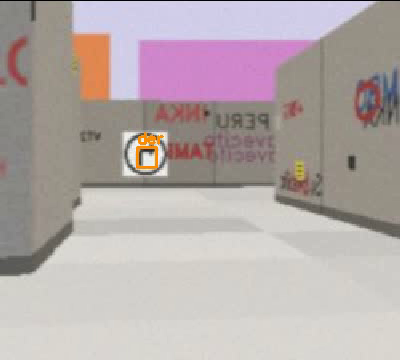
\includegraphics[width=27mm]{figuras/gen/sim_flecha.png}};
        \node[img, anchor=north west] (b) at (34,0) {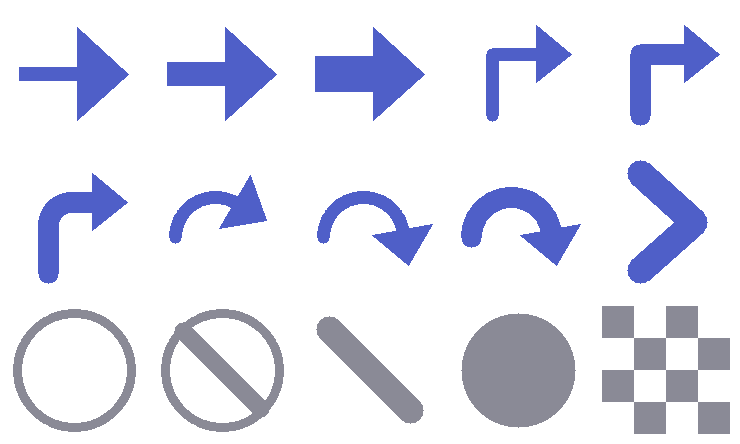
\includegraphics[width=31mm]{figuras/gen/flechas_banco.png}};
        \draw[ar] (f.east) -- (b.west);
        \node[font=\scriptsize, text=cInk, below=1.2mm of f, align=center] {lo que ve el robot};
        \node[font=\scriptsize, text=cInk, below=1.2mm of b, align=center] {se compara con 27 flechas\\dibujadas en el código\\(sin red neuronal)};
      \end{tikzpicture}\\[5mm]
      \begin{columns}[T]
        \begin{column}{0.45\linewidth}\centering
          \cifra{$\sim$88\,\%}{de las flechas detectadas en cada foto real}
        \end{column}
        \begin{column}{0.45\linewidth}\centering
          \cifra{0\,\%}{con el sentido equivocado}
        \end{column}
      \end{columns}
    \end{column}
    \begin{column}{0.47\textwidth}
      \begin{minipage}[t]{0.40\linewidth}\vspace{0pt}\centering
        \begin{tikzpicture}[x=0.95mm, y=0.95mm]
          \fill[cPaper] (0,0) rectangle (22,56);
          \draw[pared] (0,56) -- (0,0) -- (22,0) -- (22,56);
          \node[bandera] at (11,1.6) {};
          \node[foto, minimum size=2.4mm] at (0.9,34) {};
          \node[foto, minimum size=2.4mm] at (0.9,20) {};
          \node[foto, minimum size=2.4mm] at (21.1,44) {};
          \node[buscada, minimum size=2.8mm] at (21.1,26) {};
          \draw[cFila, line width=0.4pt, dash pattern=on 1pt off 1pt] (11,16) circle (7);
          \foreach \a/\n in {-45/1, 0/2, 45/3, 135/4, 180/5, -135/6}{
            \draw[cFila, line width=0.6pt, -{Stealth[length=1mm]}] (11,16) -- ++(\a:7);
            \node[circle, draw=cFila, fill=white, line width=0.5pt, inner sep=0pt, minimum size=3mm,
                  font=\fontsize{5.5}{5.5}\selectfont\bfseries, text=cFila] at ($(11,16)+(\a:11)$) {\n};}
          \draw[cInk, fill=white, line width=0.6pt] (11,16) circle (2.4);
          \draw[cInk, line width=0.8pt, -{Stealth[length=1.1mm]}] (11,16) -- (11,13.6);
          \draw[cIda, line width=1pt, -{Stealth[length=1.4mm]}] (11,63) -- (11,57);
        \end{tikzpicture}
      \end{minipage}\hfill
      \begin{minipage}[t]{0.56\linewidth}\vspace{0pt}\centering
        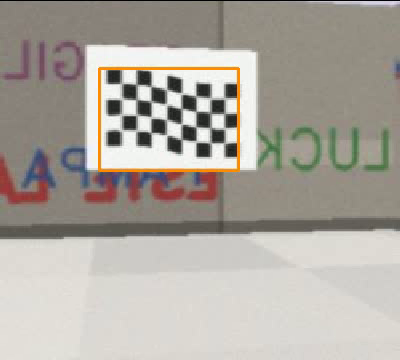
\includegraphics[width=0.85\linewidth]{figuras/gen/sim_bandera.png}\\[0.8mm]
        {\scriptsize\color{cSrc}la bandera confirma la meta\par}
      \end{minipage}
    \end{column}
  \end{columns}
\end{frame}

% =============================================================================
\section{Tarea B}
% =============================================================================

% 7 · gestos ---------------------------------------------------------------------
\begin{frame}{Tarea B: conducir solo con gestos}
  \begin{columns}[c,onlytextwidth]
    \begin{column}{0.66\textwidth}
      \gesto{der}{gira a la derecha}\hfill
      \gesto{izq}{gira a la izquierda}\hfill
      \gesto{vuelta}{media vuelta}\\[2.5mm]
      \gesto{lento}{avanza lento}\hfill
      \gesto{rapido}{avanza rápido}\hfill
      \gesto{stop}{STOP}
    \end{column}
    \begin{column}{0.31\textwidth}\centering
      \begin{tikzpicture}[x=1mm, y=1mm, node distance=2.6mm, c/.style={caja, text width=36mm, font=\footnotesize, minimum height=6.5mm}]
        \node[c] (m) {\textbf{MediaPipe}: 21 puntos};
        \node[c, below=of m] (g) {\textbf{reglas}: dedos estirados};
        \node[c, below=of g] (e) {\textbf{confirmar}: 5 de 8 cuadros};
        \node[c, below=of e, draw=cFila, line width=0.8pt] (k) {\textbf{robot}: gira, avanza o para};
        \draw[ar] (m) -- (g); \draw[ar] (g) -- (e); \draw[ar] (e) -- (k);
      \end{tikzpicture}\\[3mm]
      {\scriptsize\color{cSrc}En paralelo, la cámara del robot reconoce la cara y el QR.\par}
    \end{column}
  \end{columns}
\end{frame}

% =============================================================================
\section{Resultados}
% =============================================================================

% 8 · resultados ----------------------------------------------------------------------
\begin{frame}{Resultados}
  \begin{columns}[c,onlytextwidth]
    \begin{column}{0.44\textwidth}
      {\small\textbf{Simulador} \nota{(éxitos)}\par}\vspace{1.5mm}
      \begin{tikzpicture}
        \begin{axis}[barras, width=24mm, height=18mm, xmin=0, xmax=100, ytick={0,1},
            yticklabel style={text width=27mm},
            yticklabels={{32 circuitos al azar},{odometría con error y cámara lenta}},
            nodes near coords={\pgfmathprintnumber{\pgfplotspointmeta}\,\%}]
          \addplot[fill=cAcc, draw=none] coordinates {(100,0) (81,1)};
        \end{axis}
      \end{tikzpicture}\\[1.5mm]
      \cifra{88\,s}{mediana de la carrera completa}
      \vspace{1mm}
      {\footnotesize\color{cSrc}0 choques ni respuestas equivocadas en 48 carreras\par}
    \end{column}
    \begin{column}{0.54\textwidth}
      {\small\textbf{Robot real} \nota{(primera carrera, 19/11)}\par}\vspace{3mm}
      \begin{tikzpicture}[x=1mm, y=1mm]
        \fase{0}{0}{15}{cIda}{ida}
        \fase{0}{15}{52}{cFila}{buscar}
        \fase{0}{52}{82}{cQr}{QR}
        \fase{0}{82}{93.9}{cVuelta}{}
        \node[font=\small\bfseries, text=cInk, anchor=west] at (63,2.5) {93.9\,s};
        \draw[cInk!40, line width=0.3pt] (0,-2) -- (62,-2);
        \foreach \t in {0,30,60,90}{\draw[cInk!40] (\t*0.65,-2) -- ++(0,-0.8); \node[font=\fontsize{6.5}{7.5}\selectfont, text=cSrc, anchor=north] at (\t*0.65,-2.6) {\t\,s};}
      \end{tikzpicture}\\[3mm]
      \cifra{0 choques}{volvió a 21\,cm de A con la persona correcta}
    \end{column}
  \end{columns}
\end{frame}

% 9 · decisiones y trade-offs ----------------------------------------------------------
\begin{frame}{Decisiones de diseño}
  \vspace{3mm}
  \decision{\faMicrochip}{Todo en la Raspberry}{sin PC ni Wi-Fi}{solo $\sim$2 fotos/s}\hfill
  \decision{\faTachometer*}{Vuelta en turbo (0.45\,m/s)}{vuelta 28\,\% más rápida}{sin el límite de la Create 3}\\[8mm]
  \decision{\faDraftingCompass}{Reglas en vez de entrenar}{flechas, bandera y gestos sin modelos}{una foto sola puede fallar}\hfill
  \decision{\faSearchPlus}{Confirmar con foto HD}{no se decide con caras de 14--25\,px}{$\sim$4 s por foto HD}
\end{frame}

% =============================================================================
\section{Cierre}
% =============================================================================

% 10 · lecciones aprendidas + gracias -----------------------------------------------------
\begin{frame}{Lecciones aprendidas}
  \vspace{2mm}
  \leccion{42 \textrightarrow\ 92\,\%}{Simular con los tiempos reales del robot.}
  \leccion{9 fallos}{Probar pronto en el robot: aparecen errores que el simulador no muestra.}
  \leccion{12 \textrightarrow\ 2\,ms}{Medir antes de optimizar: el cuello era Python, no las redes.}
  \leccion{0 errores}{Ante la duda, no adivinar: sin QR seguro, se anuncia solo el nombre.}
  \vfill
  \begin{columns}[b,onlytextwidth]
    \begin{column}{0.34\textwidth}
      {\fontsize{16}{19}\selectfont\color{cAcc}¡Gracias!}\par
      \nota{\small ¿Preguntas?}
    \end{column}
    \begin{column}{0.64\textwidth}\raggedleft
      \scalebox{0.62}{\circuitoLinea}
    \end{column}
  \end{columns}
  \vspace{0.3mm}
\end{frame}

\end{document}
